\documentclass[11pt]{article}

    \usepackage[breakable]{tcolorbox}
    \usepackage{parskip} % Stop auto-indenting (to mimic markdown behaviour)
    

    % Basic figure setup, for now with no caption control since it's done
    % automatically by Pandoc (which extracts ![](path) syntax from Markdown).
    \usepackage{graphicx}
    % Maintain compatibility with old templates. Remove in nbconvert 6.0
    \let\Oldincludegraphics\includegraphics
    % Ensure that by default, figures have no caption (until we provide a
    % proper Figure object with a Caption API and a way to capture that
    % in the conversion process - todo).
    \usepackage{caption}
    \DeclareCaptionFormat{nocaption}{}
    \captionsetup{format=nocaption,aboveskip=0pt,belowskip=0pt}

    \usepackage{float}
    \floatplacement{figure}{H} % forces figures to be placed at the correct location
    \usepackage{xcolor} % Allow colors to be defined
    \usepackage{enumerate} % Needed for markdown enumerations to work
    \usepackage{geometry} % Used to adjust the document margins
    \usepackage{amsmath} % Equations
    \usepackage{amssymb} % Equations
    \usepackage{textcomp} % defines textquotesingle
    % Hack from http://tex.stackexchange.com/a/47451/13684:
    \AtBeginDocument{%
        \def\PYZsq{\textquotesingle}% Upright quotes in Pygmentized code
    }
    \usepackage{upquote} % Upright quotes for verbatim code
    \usepackage{eurosym} % defines \euro

    \usepackage{iftex}
    \ifPDFTeX
        \usepackage[T1]{fontenc}
        \IfFileExists{alphabeta.sty}{
              \usepackage{alphabeta}
          }{
              \usepackage[mathletters]{ucs}
              \usepackage[utf8x]{inputenc}
          }
    \else
        \usepackage{fontspec}
        \usepackage{unicode-math}
    \fi

    \usepackage{fancyvrb} % verbatim replacement that allows latex
    \usepackage{grffile} % extends the file name processing of package graphics
                         % to support a larger range
    \makeatletter % fix for old versions of grffile with XeLaTeX
    \@ifpackagelater{grffile}{2019/11/01}
    {
      % Do nothing on new versions
    }
    {
      \def\Gread@@xetex#1{%
        \IfFileExists{"\Gin@base".bb}%
        {\Gread@eps{\Gin@base.bb}}%
        {\Gread@@xetex@aux#1}%
      }
    }
    \makeatother
    \usepackage[Export]{adjustbox} % Used to constrain images to a maximum size
    \adjustboxset{max size={0.9\linewidth}{0.9\paperheight}}

    % The hyperref package gives us a pdf with properly built
    % internal navigation ('pdf bookmarks' for the table of contents,
    % internal cross-reference links, web links for URLs, etc.)
    \usepackage{hyperref}
    % The default LaTeX title has an obnoxious amount of whitespace. By default,
    % titling removes some of it. It also provides customization options.
    \usepackage{titling}
    \usepackage{longtable} % longtable support required by pandoc >1.10
    \usepackage{booktabs}  % table support for pandoc > 1.12.2
    \usepackage{array}     % table support for pandoc >= 2.11.3
    \usepackage{calc}      % table minipage width calculation for pandoc >= 2.11.1
    \usepackage[inline]{enumitem} % IRkernel/repr support (it uses the enumerate* environment)
    \usepackage[normalem]{ulem} % ulem is needed to support strikethroughs (\sout)
                                % normalem makes italics be italics, not underlines
    \usepackage{mathrsfs}
    

    
    % Colors for the hyperref package
    \definecolor{urlcolor}{rgb}{0,.145,.698}
    \definecolor{linkcolor}{rgb}{.71,0.21,0.01}
    \definecolor{citecolor}{rgb}{.12,.54,.11}

    % ANSI colors
    \definecolor{ansi-black}{HTML}{3E424D}
    \definecolor{ansi-black-intense}{HTML}{282C36}
    \definecolor{ansi-red}{HTML}{E75C58}
    \definecolor{ansi-red-intense}{HTML}{B22B31}
    \definecolor{ansi-green}{HTML}{00A250}
    \definecolor{ansi-green-intense}{HTML}{007427}
    \definecolor{ansi-yellow}{HTML}{DDB62B}
    \definecolor{ansi-yellow-intense}{HTML}{B27D12}
    \definecolor{ansi-blue}{HTML}{208FFB}
    \definecolor{ansi-blue-intense}{HTML}{0065CA}
    \definecolor{ansi-magenta}{HTML}{D160C4}
    \definecolor{ansi-magenta-intense}{HTML}{A03196}
    \definecolor{ansi-cyan}{HTML}{60C6C8}
    \definecolor{ansi-cyan-intense}{HTML}{258F8F}
    \definecolor{ansi-white}{HTML}{C5C1B4}
    \definecolor{ansi-white-intense}{HTML}{A1A6B2}
    \definecolor{ansi-default-inverse-fg}{HTML}{FFFFFF}
    \definecolor{ansi-default-inverse-bg}{HTML}{000000}

    % common color for the border for error outputs.
    \definecolor{outerrorbackground}{HTML}{FFDFDF}

    % commands and environments needed by pandoc snippets
    % extracted from the output of `pandoc -s`
    \providecommand{\tightlist}{%
      \setlength{\itemsep}{0pt}\setlength{\parskip}{0pt}}
    \DefineVerbatimEnvironment{Highlighting}{Verbatim}{commandchars=\\\{\}}
    % Add ',fontsize=\small' for more characters per line
    \newenvironment{Shaded}{}{}
    \newcommand{\KeywordTok}[1]{\textcolor[rgb]{0.00,0.44,0.13}{\textbf{{#1}}}}
    \newcommand{\DataTypeTok}[1]{\textcolor[rgb]{0.56,0.13,0.00}{{#1}}}
    \newcommand{\DecValTok}[1]{\textcolor[rgb]{0.25,0.63,0.44}{{#1}}}
    \newcommand{\BaseNTok}[1]{\textcolor[rgb]{0.25,0.63,0.44}{{#1}}}
    \newcommand{\FloatTok}[1]{\textcolor[rgb]{0.25,0.63,0.44}{{#1}}}
    \newcommand{\CharTok}[1]{\textcolor[rgb]{0.25,0.44,0.63}{{#1}}}
    \newcommand{\StringTok}[1]{\textcolor[rgb]{0.25,0.44,0.63}{{#1}}}
    \newcommand{\CommentTok}[1]{\textcolor[rgb]{0.38,0.63,0.69}{\textit{{#1}}}}
    \newcommand{\OtherTok}[1]{\textcolor[rgb]{0.00,0.44,0.13}{{#1}}}
    \newcommand{\AlertTok}[1]{\textcolor[rgb]{1.00,0.00,0.00}{\textbf{{#1}}}}
    \newcommand{\FunctionTok}[1]{\textcolor[rgb]{0.02,0.16,0.49}{{#1}}}
    \newcommand{\RegionMarkerTok}[1]{{#1}}
    \newcommand{\ErrorTok}[1]{\textcolor[rgb]{1.00,0.00,0.00}{\textbf{{#1}}}}
    \newcommand{\NormalTok}[1]{{#1}}

    % Additional commands for more recent versions of Pandoc
    \newcommand{\ConstantTok}[1]{\textcolor[rgb]{0.53,0.00,0.00}{{#1}}}
    \newcommand{\SpecialCharTok}[1]{\textcolor[rgb]{0.25,0.44,0.63}{{#1}}}
    \newcommand{\VerbatimStringTok}[1]{\textcolor[rgb]{0.25,0.44,0.63}{{#1}}}
    \newcommand{\SpecialStringTok}[1]{\textcolor[rgb]{0.73,0.40,0.53}{{#1}}}
    \newcommand{\ImportTok}[1]{{#1}}
    \newcommand{\DocumentationTok}[1]{\textcolor[rgb]{0.73,0.13,0.13}{\textit{{#1}}}}
    \newcommand{\AnnotationTok}[1]{\textcolor[rgb]{0.38,0.63,0.69}{\textbf{\textit{{#1}}}}}
    \newcommand{\CommentVarTok}[1]{\textcolor[rgb]{0.38,0.63,0.69}{\textbf{\textit{{#1}}}}}
    \newcommand{\VariableTok}[1]{\textcolor[rgb]{0.10,0.09,0.49}{{#1}}}
    \newcommand{\ControlFlowTok}[1]{\textcolor[rgb]{0.00,0.44,0.13}{\textbf{{#1}}}}
    \newcommand{\OperatorTok}[1]{\textcolor[rgb]{0.40,0.40,0.40}{{#1}}}
    \newcommand{\BuiltInTok}[1]{{#1}}
    \newcommand{\ExtensionTok}[1]{{#1}}
    \newcommand{\PreprocessorTok}[1]{\textcolor[rgb]{0.74,0.48,0.00}{{#1}}}
    \newcommand{\AttributeTok}[1]{\textcolor[rgb]{0.49,0.56,0.16}{{#1}}}
    \newcommand{\InformationTok}[1]{\textcolor[rgb]{0.38,0.63,0.69}{\textbf{\textit{{#1}}}}}
    \newcommand{\WarningTok}[1]{\textcolor[rgb]{0.38,0.63,0.69}{\textbf{\textit{{#1}}}}}


    % Define a nice break command that doesn't care if a line doesn't already
    % exist.
    \def\br{\hspace*{\fill} \\* }
    % Math Jax compatibility definitions
    \def\gt{>}
    \def\lt{<}
    \let\Oldtex\TeX
    \let\Oldlatex\LaTeX
    \renewcommand{\TeX}{\textrm{\Oldtex}}
    \renewcommand{\LaTeX}{\textrm{\Oldlatex}}
    % Document parameters
    % Document title
    \title{Achieving the Net-Zero Emission Target: A meta-analysis of Turkish Energy and Emission Scenarios}
    \hypertarget{by-guxf6rkem-guxfcnguxf6r-and-latife-demirtaux15f}{%
\author{By Görkem Güngör and Latife
Demirtaş}\label{by-guxf6rkem-guxfcnguxf6r-and-latife-demirtaux15f}}
    
    
    
    
% Pygments definitions
\makeatletter
\def\PY@reset{\let\PY@it=\relax \let\PY@bf=\relax%
    \let\PY@ul=\relax \let\PY@tc=\relax%
    \let\PY@bc=\relax \let\PY@ff=\relax}
\def\PY@tok#1{\csname PY@tok@#1\endcsname}
\def\PY@toks#1+{\ifx\relax#1\empty\else%
    \PY@tok{#1}\expandafter\PY@toks\fi}
\def\PY@do#1{\PY@bc{\PY@tc{\PY@ul{%
    \PY@it{\PY@bf{\PY@ff{#1}}}}}}}
\def\PY#1#2{\PY@reset\PY@toks#1+\relax+\PY@do{#2}}

\@namedef{PY@tok@w}{\def\PY@tc##1{\textcolor[rgb]{0.73,0.73,0.73}{##1}}}
\@namedef{PY@tok@c}{\let\PY@it=\textit\def\PY@tc##1{\textcolor[rgb]{0.24,0.48,0.48}{##1}}}
\@namedef{PY@tok@cp}{\def\PY@tc##1{\textcolor[rgb]{0.61,0.40,0.00}{##1}}}
\@namedef{PY@tok@k}{\let\PY@bf=\textbf\def\PY@tc##1{\textcolor[rgb]{0.00,0.50,0.00}{##1}}}
\@namedef{PY@tok@kp}{\def\PY@tc##1{\textcolor[rgb]{0.00,0.50,0.00}{##1}}}
\@namedef{PY@tok@kt}{\def\PY@tc##1{\textcolor[rgb]{0.69,0.00,0.25}{##1}}}
\@namedef{PY@tok@o}{\def\PY@tc##1{\textcolor[rgb]{0.40,0.40,0.40}{##1}}}
\@namedef{PY@tok@ow}{\let\PY@bf=\textbf\def\PY@tc##1{\textcolor[rgb]{0.67,0.13,1.00}{##1}}}
\@namedef{PY@tok@nb}{\def\PY@tc##1{\textcolor[rgb]{0.00,0.50,0.00}{##1}}}
\@namedef{PY@tok@nf}{\def\PY@tc##1{\textcolor[rgb]{0.00,0.00,1.00}{##1}}}
\@namedef{PY@tok@nc}{\let\PY@bf=\textbf\def\PY@tc##1{\textcolor[rgb]{0.00,0.00,1.00}{##1}}}
\@namedef{PY@tok@nn}{\let\PY@bf=\textbf\def\PY@tc##1{\textcolor[rgb]{0.00,0.00,1.00}{##1}}}
\@namedef{PY@tok@ne}{\let\PY@bf=\textbf\def\PY@tc##1{\textcolor[rgb]{0.80,0.25,0.22}{##1}}}
\@namedef{PY@tok@nv}{\def\PY@tc##1{\textcolor[rgb]{0.10,0.09,0.49}{##1}}}
\@namedef{PY@tok@no}{\def\PY@tc##1{\textcolor[rgb]{0.53,0.00,0.00}{##1}}}
\@namedef{PY@tok@nl}{\def\PY@tc##1{\textcolor[rgb]{0.46,0.46,0.00}{##1}}}
\@namedef{PY@tok@ni}{\let\PY@bf=\textbf\def\PY@tc##1{\textcolor[rgb]{0.44,0.44,0.44}{##1}}}
\@namedef{PY@tok@na}{\def\PY@tc##1{\textcolor[rgb]{0.41,0.47,0.13}{##1}}}
\@namedef{PY@tok@nt}{\let\PY@bf=\textbf\def\PY@tc##1{\textcolor[rgb]{0.00,0.50,0.00}{##1}}}
\@namedef{PY@tok@nd}{\def\PY@tc##1{\textcolor[rgb]{0.67,0.13,1.00}{##1}}}
\@namedef{PY@tok@s}{\def\PY@tc##1{\textcolor[rgb]{0.73,0.13,0.13}{##1}}}
\@namedef{PY@tok@sd}{\let\PY@it=\textit\def\PY@tc##1{\textcolor[rgb]{0.73,0.13,0.13}{##1}}}
\@namedef{PY@tok@si}{\let\PY@bf=\textbf\def\PY@tc##1{\textcolor[rgb]{0.64,0.35,0.47}{##1}}}
\@namedef{PY@tok@se}{\let\PY@bf=\textbf\def\PY@tc##1{\textcolor[rgb]{0.67,0.36,0.12}{##1}}}
\@namedef{PY@tok@sr}{\def\PY@tc##1{\textcolor[rgb]{0.64,0.35,0.47}{##1}}}
\@namedef{PY@tok@ss}{\def\PY@tc##1{\textcolor[rgb]{0.10,0.09,0.49}{##1}}}
\@namedef{PY@tok@sx}{\def\PY@tc##1{\textcolor[rgb]{0.00,0.50,0.00}{##1}}}
\@namedef{PY@tok@m}{\def\PY@tc##1{\textcolor[rgb]{0.40,0.40,0.40}{##1}}}
\@namedef{PY@tok@gh}{\let\PY@bf=\textbf\def\PY@tc##1{\textcolor[rgb]{0.00,0.00,0.50}{##1}}}
\@namedef{PY@tok@gu}{\let\PY@bf=\textbf\def\PY@tc##1{\textcolor[rgb]{0.50,0.00,0.50}{##1}}}
\@namedef{PY@tok@gd}{\def\PY@tc##1{\textcolor[rgb]{0.63,0.00,0.00}{##1}}}
\@namedef{PY@tok@gi}{\def\PY@tc##1{\textcolor[rgb]{0.00,0.52,0.00}{##1}}}
\@namedef{PY@tok@gr}{\def\PY@tc##1{\textcolor[rgb]{0.89,0.00,0.00}{##1}}}
\@namedef{PY@tok@ge}{\let\PY@it=\textit}
\@namedef{PY@tok@gs}{\let\PY@bf=\textbf}
\@namedef{PY@tok@gp}{\let\PY@bf=\textbf\def\PY@tc##1{\textcolor[rgb]{0.00,0.00,0.50}{##1}}}
\@namedef{PY@tok@go}{\def\PY@tc##1{\textcolor[rgb]{0.44,0.44,0.44}{##1}}}
\@namedef{PY@tok@gt}{\def\PY@tc##1{\textcolor[rgb]{0.00,0.27,0.87}{##1}}}
\@namedef{PY@tok@err}{\def\PY@bc##1{{\setlength{\fboxsep}{\string -\fboxrule}\fcolorbox[rgb]{1.00,0.00,0.00}{1,1,1}{\strut ##1}}}}
\@namedef{PY@tok@kc}{\let\PY@bf=\textbf\def\PY@tc##1{\textcolor[rgb]{0.00,0.50,0.00}{##1}}}
\@namedef{PY@tok@kd}{\let\PY@bf=\textbf\def\PY@tc##1{\textcolor[rgb]{0.00,0.50,0.00}{##1}}}
\@namedef{PY@tok@kn}{\let\PY@bf=\textbf\def\PY@tc##1{\textcolor[rgb]{0.00,0.50,0.00}{##1}}}
\@namedef{PY@tok@kr}{\let\PY@bf=\textbf\def\PY@tc##1{\textcolor[rgb]{0.00,0.50,0.00}{##1}}}
\@namedef{PY@tok@bp}{\def\PY@tc##1{\textcolor[rgb]{0.00,0.50,0.00}{##1}}}
\@namedef{PY@tok@fm}{\def\PY@tc##1{\textcolor[rgb]{0.00,0.00,1.00}{##1}}}
\@namedef{PY@tok@vc}{\def\PY@tc##1{\textcolor[rgb]{0.10,0.09,0.49}{##1}}}
\@namedef{PY@tok@vg}{\def\PY@tc##1{\textcolor[rgb]{0.10,0.09,0.49}{##1}}}
\@namedef{PY@tok@vi}{\def\PY@tc##1{\textcolor[rgb]{0.10,0.09,0.49}{##1}}}
\@namedef{PY@tok@vm}{\def\PY@tc##1{\textcolor[rgb]{0.10,0.09,0.49}{##1}}}
\@namedef{PY@tok@sa}{\def\PY@tc##1{\textcolor[rgb]{0.73,0.13,0.13}{##1}}}
\@namedef{PY@tok@sb}{\def\PY@tc##1{\textcolor[rgb]{0.73,0.13,0.13}{##1}}}
\@namedef{PY@tok@sc}{\def\PY@tc##1{\textcolor[rgb]{0.73,0.13,0.13}{##1}}}
\@namedef{PY@tok@dl}{\def\PY@tc##1{\textcolor[rgb]{0.73,0.13,0.13}{##1}}}
\@namedef{PY@tok@s2}{\def\PY@tc##1{\textcolor[rgb]{0.73,0.13,0.13}{##1}}}
\@namedef{PY@tok@sh}{\def\PY@tc##1{\textcolor[rgb]{0.73,0.13,0.13}{##1}}}
\@namedef{PY@tok@s1}{\def\PY@tc##1{\textcolor[rgb]{0.73,0.13,0.13}{##1}}}
\@namedef{PY@tok@mb}{\def\PY@tc##1{\textcolor[rgb]{0.40,0.40,0.40}{##1}}}
\@namedef{PY@tok@mf}{\def\PY@tc##1{\textcolor[rgb]{0.40,0.40,0.40}{##1}}}
\@namedef{PY@tok@mh}{\def\PY@tc##1{\textcolor[rgb]{0.40,0.40,0.40}{##1}}}
\@namedef{PY@tok@mi}{\def\PY@tc##1{\textcolor[rgb]{0.40,0.40,0.40}{##1}}}
\@namedef{PY@tok@il}{\def\PY@tc##1{\textcolor[rgb]{0.40,0.40,0.40}{##1}}}
\@namedef{PY@tok@mo}{\def\PY@tc##1{\textcolor[rgb]{0.40,0.40,0.40}{##1}}}
\@namedef{PY@tok@ch}{\let\PY@it=\textit\def\PY@tc##1{\textcolor[rgb]{0.24,0.48,0.48}{##1}}}
\@namedef{PY@tok@cm}{\let\PY@it=\textit\def\PY@tc##1{\textcolor[rgb]{0.24,0.48,0.48}{##1}}}
\@namedef{PY@tok@cpf}{\let\PY@it=\textit\def\PY@tc##1{\textcolor[rgb]{0.24,0.48,0.48}{##1}}}
\@namedef{PY@tok@c1}{\let\PY@it=\textit\def\PY@tc##1{\textcolor[rgb]{0.24,0.48,0.48}{##1}}}
\@namedef{PY@tok@cs}{\let\PY@it=\textit\def\PY@tc##1{\textcolor[rgb]{0.24,0.48,0.48}{##1}}}

\def\PYZbs{\char`\\}
\def\PYZus{\char`\_}
\def\PYZob{\char`\{}
\def\PYZcb{\char`\}}
\def\PYZca{\char`\^}
\def\PYZam{\char`\&}
\def\PYZlt{\char`\<}
\def\PYZgt{\char`\>}
\def\PYZsh{\char`\#}
\def\PYZpc{\char`\%}
\def\PYZdl{\char`\$}
\def\PYZhy{\char`\-}
\def\PYZsq{\char`\'}
\def\PYZdq{\char`\"}
\def\PYZti{\char`\~}
% for compatibility with earlier versions
\def\PYZat{@}
\def\PYZlb{[}
\def\PYZrb{]}
\makeatother


    % For linebreaks inside Verbatim environment from package fancyvrb.
    \makeatletter
        \newbox\Wrappedcontinuationbox
        \newbox\Wrappedvisiblespacebox
        \newcommand*\Wrappedvisiblespace {\textcolor{red}{\textvisiblespace}}
        \newcommand*\Wrappedcontinuationsymbol {\textcolor{red}{\llap{\tiny$\m@th\hookrightarrow$}}}
        \newcommand*\Wrappedcontinuationindent {3ex }
        \newcommand*\Wrappedafterbreak {\kern\Wrappedcontinuationindent\copy\Wrappedcontinuationbox}
        % Take advantage of the already applied Pygments mark-up to insert
        % potential linebreaks for TeX processing.
        %        {, <, #, %, $, ' and ": go to next line.
        %        _, }, ^, &, >, - and ~: stay at end of broken line.
        % Use of \textquotesingle for straight quote.
        \newcommand*\Wrappedbreaksatspecials {%
            \def\PYGZus{\discretionary{\char`\_}{\Wrappedafterbreak}{\char`\_}}%
            \def\PYGZob{\discretionary{}{\Wrappedafterbreak\char`\{}{\char`\{}}%
            \def\PYGZcb{\discretionary{\char`\}}{\Wrappedafterbreak}{\char`\}}}%
            \def\PYGZca{\discretionary{\char`\^}{\Wrappedafterbreak}{\char`\^}}%
            \def\PYGZam{\discretionary{\char`\&}{\Wrappedafterbreak}{\char`\&}}%
            \def\PYGZlt{\discretionary{}{\Wrappedafterbreak\char`\<}{\char`\<}}%
            \def\PYGZgt{\discretionary{\char`\>}{\Wrappedafterbreak}{\char`\>}}%
            \def\PYGZsh{\discretionary{}{\Wrappedafterbreak\char`\#}{\char`\#}}%
            \def\PYGZpc{\discretionary{}{\Wrappedafterbreak\char`\%}{\char`\%}}%
            \def\PYGZdl{\discretionary{}{\Wrappedafterbreak\char`\$}{\char`\$}}%
            \def\PYGZhy{\discretionary{\char`\-}{\Wrappedafterbreak}{\char`\-}}%
            \def\PYGZsq{\discretionary{}{\Wrappedafterbreak\textquotesingle}{\textquotesingle}}%
            \def\PYGZdq{\discretionary{}{\Wrappedafterbreak\char`\"}{\char`\"}}%
            \def\PYGZti{\discretionary{\char`\~}{\Wrappedafterbreak}{\char`\~}}%
        }
        % Some characters . , ; ? ! / are not pygmentized.
        % This macro makes them "active" and they will insert potential linebreaks
        \newcommand*\Wrappedbreaksatpunct {%
            \lccode`\~`\.\lowercase{\def~}{\discretionary{\hbox{\char`\.}}{\Wrappedafterbreak}{\hbox{\char`\.}}}%
            \lccode`\~`\,\lowercase{\def~}{\discretionary{\hbox{\char`\,}}{\Wrappedafterbreak}{\hbox{\char`\,}}}%
            \lccode`\~`\;\lowercase{\def~}{\discretionary{\hbox{\char`\;}}{\Wrappedafterbreak}{\hbox{\char`\;}}}%
            \lccode`\~`\:\lowercase{\def~}{\discretionary{\hbox{\char`\:}}{\Wrappedafterbreak}{\hbox{\char`\:}}}%
            \lccode`\~`\?\lowercase{\def~}{\discretionary{\hbox{\char`\?}}{\Wrappedafterbreak}{\hbox{\char`\?}}}%
            \lccode`\~`\!\lowercase{\def~}{\discretionary{\hbox{\char`\!}}{\Wrappedafterbreak}{\hbox{\char`\!}}}%
            \lccode`\~`\/\lowercase{\def~}{\discretionary{\hbox{\char`\/}}{\Wrappedafterbreak}{\hbox{\char`\/}}}%
            \catcode`\.\active
            \catcode`\,\active
            \catcode`\;\active
            \catcode`\:\active
            \catcode`\?\active
            \catcode`\!\active
            \catcode`\/\active
            \lccode`\~`\~
        }
    \makeatother

    \let\OriginalVerbatim=\Verbatim
    \makeatletter
    \renewcommand{\Verbatim}[1][1]{%
        %\parskip\z@skip
        \sbox\Wrappedcontinuationbox {\Wrappedcontinuationsymbol}%
        \sbox\Wrappedvisiblespacebox {\FV@SetupFont\Wrappedvisiblespace}%
        \def\FancyVerbFormatLine ##1{\hsize\linewidth
            \vtop{\raggedright\hyphenpenalty\z@\exhyphenpenalty\z@
                \doublehyphendemerits\z@\finalhyphendemerits\z@
                \strut ##1\strut}%
        }%
        % If the linebreak is at a space, the latter will be displayed as visible
        % space at end of first line, and a continuation symbol starts next line.
        % Stretch/shrink are however usually zero for typewriter font.
        \def\FV@Space {%
            \nobreak\hskip\z@ plus\fontdimen3\font minus\fontdimen4\font
            \discretionary{\copy\Wrappedvisiblespacebox}{\Wrappedafterbreak}
            {\kern\fontdimen2\font}%
        }%

        % Allow breaks at special characters using \PYG... macros.
        \Wrappedbreaksatspecials
        % Breaks at punctuation characters . , ; ? ! and / need catcode=\active
        \OriginalVerbatim[#1,codes*=\Wrappedbreaksatpunct]%
    }
    \makeatother

    % Exact colors from NB
    \definecolor{incolor}{HTML}{303F9F}
    \definecolor{outcolor}{HTML}{D84315}
    \definecolor{cellborder}{HTML}{CFCFCF}
    \definecolor{cellbackground}{HTML}{F7F7F7}

    % prompt
    \makeatletter
    \newcommand{\boxspacing}{\kern\kvtcb@left@rule\kern\kvtcb@boxsep}
    \makeatother
    \newcommand{\prompt}[4]{
        {\ttfamily\llap{{\color{#2}[#3]:\hspace{3pt}#4}}\vspace{-\baselineskip}}
    }
    

    
    % Prevent overflowing lines due to hard-to-break entities
    \sloppy
    % Setup hyperref package
    \hypersetup{
      breaklinks=true,  % so long urls are correctly broken across lines
      colorlinks=true,
      urlcolor=urlcolor,
      linkcolor=linkcolor,
      citecolor=citecolor,
      }
    % Slightly bigger margins than the latex defaults
    
    \geometry{verbose,tmargin=1in,bmargin=1in,lmargin=1in,rmargin=1in}
    
    

\begin{document}
    
    \maketitle
    
    

    
    \begin{figure}
\centering

\includegraphics{hulogo.png}
\caption{hulogo.png}
\end{figure}

\hypertarget{meta-analysis-of-turkish-energy-and-climate-pathways}{%
\section{\texorpdfstring{ Meta-analysis of Turkish Energy and Climate
Pathways
}{ Meta-analysis of Turkish Energy and Climate Pathways }}\label{meta-analysis-of-turkish-energy-and-climate-pathways}}

    \hypertarget{scope-and-feature-overview}{%
\subsection{Scope and feature
overview}\label{scope-and-feature-overview}}

The \textbf{Türkiye National Energy Plan} (TUEP) modeling horizon is
2035 based on the net-zero target in 2053.

The \textbf{pyam} package is used for analyzing, visualizing and working
with timeseries data following the format established by the
\emph{Integrated Assessment Modeling Consortium}
(\href{https://www.iamconsortium.org}{IAMC});
\href{https://pyam-iamc.readthedocs.io/en/stable/data.html}{read the
docs} for more information.

    \hypertarget{highlights}{%
\subsection{Highlights}\label{highlights}}

The main themes for the \textbf{Türkiye National Energy Plan} and the
\textbf{Türkiye Hydrogen Strategy and Road-Map} modeling horizon 2035
are:

\begin{itemize}
\tightlist
\item
  Final renewable energy includes solar, biomass and geothermal
\item
  Hydrogen and synthetic methane are clean fuels
\item
  Hydrogen is produced in the electrolyser, whereas DAC using CCS is
  optional for producing synthetic methane after 2035
\item
  Final natural gas is blended by 3.5\% with hydrogen for final sectoral
  demand after 2035
\item
  Secondary renewable electricity includes solar, wind, hydro, biomass
  and geothermal
\item
  Although the emissions are not specified, the plan is based on the
  net-zero carbon emission target for 2053
\item
  Battery storage has 2 hours charging period.
\end{itemize}

    \hypertarget{capacity-projections}{%
\subsection{Capacity projections}\label{capacity-projections}}

\begin{longtable}[]{@{}
  >{\raggedright\arraybackslash}p{(\columnwidth - 8\tabcolsep) * \real{0.4848}}
  >{\raggedright\arraybackslash}p{(\columnwidth - 8\tabcolsep) * \real{0.1515}}
  >{\raggedright\arraybackslash}p{(\columnwidth - 8\tabcolsep) * \real{0.1212}}
  >{\raggedright\arraybackslash}p{(\columnwidth - 8\tabcolsep) * \real{0.1212}}
  >{\raggedright\arraybackslash}p{(\columnwidth - 8\tabcolsep) * \real{0.1212}}@{}}
\toprule()
\begin{minipage}[b]{\linewidth}\raggedright
Installed capacity
\end{minipage} & \begin{minipage}[b]{\linewidth}\raggedright
unit
\end{minipage} & \begin{minipage}[b]{\linewidth}\raggedright
2030
\end{minipage} & \begin{minipage}[b]{\linewidth}\raggedright
2035
\end{minipage} & \begin{minipage}[b]{\linewidth}\raggedright
2055
\end{minipage} \\
\midrule()
\endhead
Solar power & GW & & 52.9 (59.7\hyperref[fn1-back]{1}) & \\
Wind power & GW & & 29.6 (50.1\hyperref[fn1-back]{1}) & \\
Nuclear power & GW & & 7.2 (4.8\hyperref[fn1-back]{1}) & \\
New installed capacity & GW & & 96.9 & \\
Total installed capacity & GW & & 189.7 (202.1\hyperref[fn1-back]{1})
& \\
Battery storage & GW & & 7.5 & \\
Electrolyser & GW & 1.9 & 5.0 & 70.0 \\
Demand side management & GW & 0.9 & 1.7 & \\
\bottomrule()
\end{longtable}

\hyperref[fn1-back]{1} Capacity projections of Istanbul Policy Center
for Net-Zero Scenario

    \hypertarget{data}{%
\subsection{Data}\label{data}}

The timeseries data used in this notebook are manually assembled from
official reports. The main official report is the \emph{Türkiye National
Energy Plan}
(\href{https://enerji.gov.tr/Media/Dizin/EIGM/tr/Raporlar/TUEP/T\%C3\%BCrkiye_National_Energy_Plan.pdf}{TUEP})
of the Ministry of Energy and Natural Resources.

\hypertarget{scenarios-in-the-data}{%
\subsubsection{Scenarios in the data}\label{scenarios-in-the-data}}

The scenarios included in the official reports are:

\begin{itemize}
\tightlist
\item
  Energy Security Scenario from the Ministry of Energy and Natural
  Resources (2023) \emph{Türkiye National Energy Plan}
\item
  Baseline and Net-Zero Scenarios from Istanbul Policy Center (2021)
  \emph{Turkey's Decarbonization Pathway}
\item
  Baseline, Optimistic and Pessimistic Scenarios from TÜBİTAK-MAM (2012)
  \emph{Mitigation / Adaptation scenarios and Climate Change policy
  portfolios for Turkey}
\end{itemize}

This notebook is intended for meta-analysis of Turkish energy and
climate pathways from the literature.

\begin{center}\rule{0.5\linewidth}{0.5pt}\end{center}

    \begin{tcolorbox}[breakable, size=fbox, boxrule=1pt, pad at break*=1mm,colback=cellbackground, colframe=cellborder]
\prompt{In}{incolor}{1}{\boxspacing}
\begin{Verbatim}[commandchars=\\\{\}]
\PY{k+kn}{import} \PY{n+nn}{numpy} \PY{k}{as} \PY{n+nn}{np}
\PY{k+kn}{import} \PY{n+nn}{pyam}
\PY{k+kn}{import} \PY{n+nn}{matplotlib}\PY{n+nn}{.}\PY{n+nn}{pyplot} \PY{k}{as} \PY{n+nn}{plt}
\end{Verbatim}
\end{tcolorbox}

    
    \begin{Verbatim}[commandchars=\\\{\}]
<IPython.core.display.Javascript object>
    \end{Verbatim}

    
    \hypertarget{import-data-from-file-and-inspect-the-scenario}{%
\subsection{Import data from file and inspect the
scenario}\label{import-data-from-file-and-inspect-the-scenario}}

We import the snapshot of the timeseries data from the file
\texttt{data.csv}.

If you haven't cloned the
\href{https://github.com/gorkemgungormetu/turkish_energy_and_climate_pathways.git}{GitHub
repository} to your machine, you can download the file from GitHub
\href{https://github.com/gorkemgungormetu/turkish_energy_and_climate_pathways/data.csv}{data}.\\
Make sure to place the file in the same folder as this notebook.

    \begin{tcolorbox}[breakable, size=fbox, boxrule=1pt, pad at break*=1mm,colback=cellbackground, colframe=cellborder]
\prompt{In}{incolor}{2}{\boxspacing}
\begin{Verbatim}[commandchars=\\\{\}]
\PY{n}{df} \PY{o}{=} \PY{n}{pyam}\PY{o}{.}\PY{n}{IamDataFrame}\PY{p}{(}\PY{n}{data}\PY{o}{=}\PY{l+s+s1}{\PYZsq{}}\PY{l+s+s1}{data.csv}\PY{l+s+s1}{\PYZsq{}}\PY{p}{)}
\end{Verbatim}
\end{tcolorbox}

    \begin{Verbatim}[commandchars=\\\{\}]
pyam - INFO: Running in a notebook, setting up a basic logging at level INFO
pyam.core - INFO: Reading file data.csv
    \end{Verbatim}

    As a first step, we show an overview of the \textbf{IamDataFrame}
content by simply calling \texttt{df} (alternatively, you can use
\texttt{print(df)} or
\href{https://pyam-iamc.readthedocs.io/en/stable/api/iamdataframe.html\#pyam.IamDataFrame.info}{df.info()}).

This function returns a concise (abbreviated) overview of the index
dimensions and the qualitative/quantitative meta indicators (see an
explanation of indicators below).

    \begin{tcolorbox}[breakable, size=fbox, boxrule=1pt, pad at break*=1mm,colback=cellbackground, colframe=cellborder]
\prompt{In}{incolor}{3}{\boxspacing}
\begin{Verbatim}[commandchars=\\\{\}]
\PY{n}{df}
\end{Verbatim}
\end{tcolorbox}

            \begin{tcolorbox}[breakable, size=fbox, boxrule=.5pt, pad at break*=1mm, opacityfill=0]
\prompt{Out}{outcolor}{3}{\boxspacing}
\begin{Verbatim}[commandchars=\\\{\}]
<class 'pyam.core.IamDataFrame'>
Index:
 * model    : Gungor (2020), IPC (2021), MENR (2006), MENR (2023), TUBITAK
(2012) (5)
 * scenario : Baseline Scenario, CO2 Scenario, {\ldots} SSP3-RCP3.4-FIT (15)
Timeseries data coordinates:
   region   : Turkey (1)
   variable : Emissions|CO2, Final Energy, {\ldots} Secondary Energy|Electricity|Wind
(47)
   unit     : MW, Mt CO2/yr, Mtoe/yr, TWh/yr (4)
   year     : 2010, 2020, 2030, 2040, 2050, 2055, 2070 (7)
   type     : CGE, Linear Programming, Market Based Simulation, Regression
Analysis (4)
Meta indicators:
   exclude (bool) False (1)
\end{Verbatim}
\end{tcolorbox}
        
    In the following cells, we display the lists of all models, scenarios,
regions, and the mapping of variables to units in the snapshot.

    \begin{tcolorbox}[breakable, size=fbox, boxrule=1pt, pad at break*=1mm,colback=cellbackground, colframe=cellborder]
\prompt{In}{incolor}{4}{\boxspacing}
\begin{Verbatim}[commandchars=\\\{\}]
\PY{n}{df}\PY{o}{.}\PY{n}{model}
\end{Verbatim}
\end{tcolorbox}

            \begin{tcolorbox}[breakable, size=fbox, boxrule=.5pt, pad at break*=1mm, opacityfill=0]
\prompt{Out}{outcolor}{4}{\boxspacing}
\begin{Verbatim}[commandchars=\\\{\}]
['Gungor (2020)', 'IPC (2021)', 'MENR (2006)', 'MENR (2023)', 'TUBITAK (2012)']
\end{Verbatim}
\end{tcolorbox}
        
    \begin{tcolorbox}[breakable, size=fbox, boxrule=1pt, pad at break*=1mm,colback=cellbackground, colframe=cellborder]
\prompt{In}{incolor}{5}{\boxspacing}
\begin{Verbatim}[commandchars=\\\{\}]
\PY{n}{df}\PY{o}{.}\PY{n}{scenario}
\end{Verbatim}
\end{tcolorbox}

            \begin{tcolorbox}[breakable, size=fbox, boxrule=.5pt, pad at break*=1mm, opacityfill=0]
\prompt{Out}{outcolor}{5}{\boxspacing}
\begin{Verbatim}[commandchars=\\\{\}]
['Baseline Scenario',
 'CO2 Scenario',
 'Cogeneration Scenario',
 'Demand Efficiency Scenario',
 'Low Demand Scenario',
 'Net-Zero Scenario',
 'No-Nuclear Scenario',
 'Optimistic Scenario',
 'Pessimistic Scenario',
 'SSP1-Baseline-FIT',
 'SSP1-RCP2.6-FIT',
 'SSP2-Baseline-FIT',
 'SSP2-RCP2.6-FIT',
 'SSP3-Baseline-FIT',
 'SSP3-RCP3.4-FIT']
\end{Verbatim}
\end{tcolorbox}
        
    \begin{tcolorbox}[breakable, size=fbox, boxrule=1pt, pad at break*=1mm,colback=cellbackground, colframe=cellborder]
\prompt{In}{incolor}{6}{\boxspacing}
\begin{Verbatim}[commandchars=\\\{\}]
\PY{n}{df}\PY{o}{.}\PY{n}{region}
\end{Verbatim}
\end{tcolorbox}

            \begin{tcolorbox}[breakable, size=fbox, boxrule=.5pt, pad at break*=1mm, opacityfill=0]
\prompt{Out}{outcolor}{6}{\boxspacing}
\begin{Verbatim}[commandchars=\\\{\}]
['Turkey']
\end{Verbatim}
\end{tcolorbox}
        
    \begin{tcolorbox}[breakable, size=fbox, boxrule=1pt, pad at break*=1mm,colback=cellbackground, colframe=cellborder]
\prompt{In}{incolor}{7}{\boxspacing}
\begin{Verbatim}[commandchars=\\\{\}]
\PY{n}{df}\PY{o}{.}\PY{n}{unit\PYZus{}mapping}
\end{Verbatim}
\end{tcolorbox}

            \begin{tcolorbox}[breakable, size=fbox, boxrule=.5pt, pad at break*=1mm, opacityfill=0]
\prompt{Out}{outcolor}{7}{\boxspacing}
\begin{Verbatim}[commandchars=\\\{\}]
\{'Emissions|CO2': 'Mt CO2/yr',
 'Final Energy': 'Mtoe/yr',
 'Final Energy|Agriculture': 'Mtoe/yr',
 'Final Energy|Agriculture|Electricity': 'TWh/yr',
 'Final Energy|Commercial': 'Mtoe/yr',
 'Final Energy|Electricity': ['TWh/yr', 'Mtoe/yr'],
 'Final Energy|Gases': 'Mtoe/yr',
 'Final Energy|Heat': 'Mtoe/yr',
 'Final Energy|Hydrogen': 'TWh/yr',
 'Final Energy|Industry': 'Mtoe/yr',
 'Final Energy|Industry|Electricity': 'TWh/yr',
 'Final Energy|Liquids': 'Mtoe/yr',
 'Final Energy|Non-Energy': 'Mtoe/yr',
 'Final Energy|Other': 'Mtoe/yr',
 'Final Energy|Renewables': 'Mtoe/yr',
 'Final Energy|Residential': 'Mtoe/yr',
 'Final Energy|Residential|Electricity': 'TWh/yr',
 'Final Energy|Services|Electricity': 'TWh/yr',
 'Final Energy|Solids': 'Mtoe/yr',
 'Final Energy|Transportation': 'Mtoe/yr',
 'Final Energy|Transportation|Electricity': 'TWh/yr',
 'Primary Energy': ['MW', 'Mtoe/yr'],
 'Primary Energy|Biomass': 'Mtoe/yr',
 'Primary Energy|Coal': 'Mtoe/yr',
 'Primary Energy|Gas': 'Mtoe/yr',
 'Primary Energy|Geothermal|Electricity': 'Mtoe/yr',
 'Primary Energy|Geothermal|Heat': 'Mtoe/yr',
 'Primary Energy|Hydro': 'Mtoe/yr',
 'Primary Energy|Nuclear': 'Mtoe/yr',
 'Primary Energy|Oil': 'Mtoe/yr',
 'Primary Energy|Renewables': 'Mtoe/yr',
 'Primary Energy|Solar': 'Mtoe/yr',
 'Primary Energy|Wind': 'Mtoe/yr',
 'Secondary Energy|Electricity': 'TWh/yr',
 'Secondary Energy|Electricity|Coal': 'TWh/yr',
 'Secondary Energy|Electricity|Fossil': 'TWh/yr',
 'Secondary Energy|Electricity|Gas': 'TWh/yr',
 'Secondary Energy|Electricity|Gases': 'TWh/yr',
 'Secondary Energy|Electricity|Hydro': 'TWh/yr',
 'Secondary Energy|Electricity|Nuclear': 'TWh/yr',
 'Secondary Energy|Electricity|Oil': 'TWh/yr',
 'Secondary Energy|Electricity|Other': 'TWh/yr',
 'Secondary Energy|Electricity|Renewables': 'TWh/yr',
 'Secondary Energy|Electricity|Renewables|Solar': 'TWh/yr',
 'Secondary Energy|Electricity|Renewables|Wind': 'TWh/yr',
 'Secondary Energy|Electricity|Solar': 'TWh/yr',
 'Secondary Energy|Electricity|Wind': 'TWh/yr'\}
\end{Verbatim}
\end{tcolorbox}
        
    We convert the units \textbf{Mtoe/yr} and \textbf{TWh/yr} to
\textbf{EJ/yr} compliant with the IAMC template.

    \begin{tcolorbox}[breakable, size=fbox, boxrule=1pt, pad at break*=1mm,colback=cellbackground, colframe=cellborder]
\prompt{In}{incolor}{8}{\boxspacing}
\begin{Verbatim}[commandchars=\\\{\}]
\PY{n}{df}\PY{o}{.}\PY{n}{convert\PYZus{}unit}\PY{p}{(}\PY{l+s+s1}{\PYZsq{}}\PY{l+s+s1}{Mtoe/yr}\PY{l+s+s1}{\PYZsq{}}\PY{p}{,} \PY{n}{to}\PY{o}{=}\PY{l+s+s1}{\PYZsq{}}\PY{l+s+s1}{EJ/yr}\PY{l+s+s1}{\PYZsq{}}\PY{p}{,} \PY{n}{inplace}\PY{o}{=}\PY{k+kc}{True}\PY{p}{)}
\PY{n}{df}\PY{o}{.}\PY{n}{convert\PYZus{}unit}\PY{p}{(}\PY{l+s+s1}{\PYZsq{}}\PY{l+s+s1}{TWh/yr}\PY{l+s+s1}{\PYZsq{}}\PY{p}{,} \PY{n}{to}\PY{o}{=}\PY{l+s+s1}{\PYZsq{}}\PY{l+s+s1}{EJ/yr}\PY{l+s+s1}{\PYZsq{}}\PY{p}{,} \PY{n}{inplace}\PY{o}{=}\PY{k+kc}{True}\PY{p}{)}
\PY{n}{df}\PY{o}{.}\PY{n}{convert\PYZus{}unit}\PY{p}{(}\PY{l+s+s1}{\PYZsq{}}\PY{l+s+s1}{MW}\PY{l+s+s1}{\PYZsq{}}\PY{p}{,} \PY{n}{to}\PY{o}{=}\PY{l+s+s1}{\PYZsq{}}\PY{l+s+s1}{EJ/yr}\PY{l+s+s1}{\PYZsq{}}\PY{p}{,} \PY{n}{inplace}\PY{o}{=}\PY{k+kc}{True}\PY{p}{)}
\end{Verbatim}
\end{tcolorbox}

    \begin{tcolorbox}[breakable, size=fbox, boxrule=1pt, pad at break*=1mm,colback=cellbackground, colframe=cellborder]
\prompt{In}{incolor}{9}{\boxspacing}
\begin{Verbatim}[commandchars=\\\{\}]
\PY{n}{df}\PY{o}{.}\PY{n}{unit\PYZus{}mapping}
\end{Verbatim}
\end{tcolorbox}

            \begin{tcolorbox}[breakable, size=fbox, boxrule=.5pt, pad at break*=1mm, opacityfill=0]
\prompt{Out}{outcolor}{9}{\boxspacing}
\begin{Verbatim}[commandchars=\\\{\}]
\{'Emissions|CO2': 'Mt CO2/yr',
 'Final Energy': 'EJ/yr',
 'Final Energy|Agriculture': 'EJ/yr',
 'Final Energy|Agriculture|Electricity': 'EJ/yr',
 'Final Energy|Commercial': 'EJ/yr',
 'Final Energy|Electricity': 'EJ/yr',
 'Final Energy|Gases': 'EJ/yr',
 'Final Energy|Heat': 'EJ/yr',
 'Final Energy|Hydrogen': 'EJ/yr',
 'Final Energy|Industry': 'EJ/yr',
 'Final Energy|Industry|Electricity': 'EJ/yr',
 'Final Energy|Liquids': 'EJ/yr',
 'Final Energy|Non-Energy': 'EJ/yr',
 'Final Energy|Other': 'EJ/yr',
 'Final Energy|Renewables': 'EJ/yr',
 'Final Energy|Residential': 'EJ/yr',
 'Final Energy|Residential|Electricity': 'EJ/yr',
 'Final Energy|Services|Electricity': 'EJ/yr',
 'Final Energy|Solids': 'EJ/yr',
 'Final Energy|Transportation': 'EJ/yr',
 'Final Energy|Transportation|Electricity': 'EJ/yr',
 'Primary Energy': 'EJ/yr',
 'Primary Energy|Biomass': 'EJ/yr',
 'Primary Energy|Coal': 'EJ/yr',
 'Primary Energy|Gas': 'EJ/yr',
 'Primary Energy|Geothermal|Electricity': 'EJ/yr',
 'Primary Energy|Geothermal|Heat': 'EJ/yr',
 'Primary Energy|Hydro': 'EJ/yr',
 'Primary Energy|Nuclear': 'EJ/yr',
 'Primary Energy|Oil': 'EJ/yr',
 'Primary Energy|Renewables': 'EJ/yr',
 'Primary Energy|Solar': 'EJ/yr',
 'Primary Energy|Wind': 'EJ/yr',
 'Secondary Energy|Electricity': 'EJ/yr',
 'Secondary Energy|Electricity|Coal': 'EJ/yr',
 'Secondary Energy|Electricity|Fossil': 'EJ/yr',
 'Secondary Energy|Electricity|Gas': 'EJ/yr',
 'Secondary Energy|Electricity|Gases': 'EJ/yr',
 'Secondary Energy|Electricity|Hydro': 'EJ/yr',
 'Secondary Energy|Electricity|Nuclear': 'EJ/yr',
 'Secondary Energy|Electricity|Oil': 'EJ/yr',
 'Secondary Energy|Electricity|Other': 'EJ/yr',
 'Secondary Energy|Electricity|Renewables': 'EJ/yr',
 'Secondary Energy|Electricity|Renewables|Solar': 'EJ/yr',
 'Secondary Energy|Electricity|Renewables|Wind': 'EJ/yr',
 'Secondary Energy|Electricity|Solar': 'EJ/yr',
 'Secondary Energy|Electricity|Wind': 'EJ/yr'\}
\end{Verbatim}
\end{tcolorbox}
        
    \hypertarget{apply-filters-to-the-ensemble-and-display-the-timeseries-data}{%
\subsection{Apply filters to the ensemble and display the timeseries
data}\label{apply-filters-to-the-ensemble-and-display-the-timeseries-data}}

A selection of the timeseries data of an \textbf{IamDataFrame} can be
obtained by applying the
\href{https://pyam-iamc.readthedocs.io/en/stable/api/iamdataframe.html\#pyam.IamDataFrame.filter}{filter()}
function, which takes keyword-arguments of criteria. The function
returns a down-selected clone of the \textbf{IamDataFrame} instance.

\hypertarget{filtering-by-model-names-scenarios-and-regions}{%
\subsubsection{Filtering by model names, scenarios and
regions}\label{filtering-by-model-names-scenarios-and-regions}}

The feature for filtering by \textbf{model, scenario or region} are
implemented using exact string matching, where \texttt{*} can be used as
a wildcard.

First, we want to display the list of all scenarios in TUEP.

\begin{quote}
Applying the filter argument
\texttt{model=\textquotesingle{}MENR\textquotesingle{}} will return an
empty array\\
(because the model in the data is actually called \textbf{MENR (2023)})
\end{quote}

    \begin{tcolorbox}[breakable, size=fbox, boxrule=1pt, pad at break*=1mm,colback=cellbackground, colframe=cellborder]
\prompt{In}{incolor}{10}{\boxspacing}
\begin{Verbatim}[commandchars=\\\{\}]
\PY{n}{df}\PY{o}{.}\PY{n}{filter}\PY{p}{(}\PY{n}{model}\PY{o}{=}\PY{l+s+s1}{\PYZsq{}}\PY{l+s+s1}{MENR}\PY{l+s+s1}{\PYZsq{}}\PY{p}{)}\PY{o}{.}\PY{n}{scenario}
\end{Verbatim}
\end{tcolorbox}

    \begin{Verbatim}[commandchars=\\\{\}]
pyam.core - WARNING: Filtered IamDataFrame is empty!
    \end{Verbatim}

            \begin{tcolorbox}[breakable, size=fbox, boxrule=.5pt, pad at break*=1mm, opacityfill=0]
\prompt{Out}{outcolor}{10}{\boxspacing}
\begin{Verbatim}[commandchars=\\\{\}]
[]
\end{Verbatim}
\end{tcolorbox}
        
    Filtering for \texttt{model=\textquotesingle{}MENR*\textquotesingle{}}
will return all scenarios provided by the \textbf{Ministry of Energy and
Natural Resources}.

    \begin{tcolorbox}[breakable, size=fbox, boxrule=1pt, pad at break*=1mm,colback=cellbackground, colframe=cellborder]
\prompt{In}{incolor}{11}{\boxspacing}
\begin{Verbatim}[commandchars=\\\{\}]
\PY{n}{df}\PY{o}{.}\PY{n}{filter}\PY{p}{(}\PY{n}{model}\PY{o}{=}\PY{l+s+s1}{\PYZsq{}}\PY{l+s+s1}{MENR*}\PY{l+s+s1}{\PYZsq{}}\PY{p}{)}\PY{o}{.}\PY{n}{scenario}
\end{Verbatim}
\end{tcolorbox}

            \begin{tcolorbox}[breakable, size=fbox, boxrule=.5pt, pad at break*=1mm, opacityfill=0]
\prompt{Out}{outcolor}{11}{\boxspacing}
\begin{Verbatim}[commandchars=\\\{\}]
['Baseline Scenario',
 'Cogeneration Scenario',
 'Demand Efficiency Scenario',
 'Low Demand Scenario',
 'No-Nuclear Scenario',
 'CO2 Scenario']
\end{Verbatim}
\end{tcolorbox}
        
    \hypertarget{inverting-the-selection}{%
\subsubsection{Inverting the selection}\label{inverting-the-selection}}

Using the keyword \texttt{keep=False} allows you to select the inverse
of the filter arguments. We can see that our data only contains
information for region \emph{Turkey}.

    \begin{tcolorbox}[breakable, size=fbox, boxrule=1pt, pad at break*=1mm,colback=cellbackground, colframe=cellborder]
\prompt{In}{incolor}{12}{\boxspacing}
\begin{Verbatim}[commandchars=\\\{\}]
\PY{n}{df}\PY{o}{.}\PY{n}{filter}\PY{p}{(}\PY{n}{region}\PY{o}{=}\PY{l+s+s1}{\PYZsq{}}\PY{l+s+s1}{Turkey}\PY{l+s+s1}{\PYZsq{}}\PY{p}{)}\PY{o}{.}\PY{n}{region}
\end{Verbatim}
\end{tcolorbox}

            \begin{tcolorbox}[breakable, size=fbox, boxrule=.5pt, pad at break*=1mm, opacityfill=0]
\prompt{Out}{outcolor}{12}{\boxspacing}
\begin{Verbatim}[commandchars=\\\{\}]
['Turkey']
\end{Verbatim}
\end{tcolorbox}
        
    \begin{tcolorbox}[breakable, size=fbox, boxrule=1pt, pad at break*=1mm,colback=cellbackground, colframe=cellborder]
\prompt{In}{incolor}{13}{\boxspacing}
\begin{Verbatim}[commandchars=\\\{\}]
\PY{n}{df}\PY{o}{.}\PY{n}{filter}\PY{p}{(}\PY{n}{region}\PY{o}{=}\PY{l+s+s1}{\PYZsq{}}\PY{l+s+s1}{Turkey}\PY{l+s+s1}{\PYZsq{}}\PY{p}{,} \PY{n}{keep}\PY{o}{=}\PY{k+kc}{False}\PY{p}{)}\PY{o}{.}\PY{n}{region}
\end{Verbatim}
\end{tcolorbox}

    \begin{Verbatim}[commandchars=\\\{\}]
pyam.core - WARNING: Filtered IamDataFrame is empty!
    \end{Verbatim}

            \begin{tcolorbox}[breakable, size=fbox, boxrule=.5pt, pad at break*=1mm, opacityfill=0]
\prompt{Out}{outcolor}{13}{\boxspacing}
\begin{Verbatim}[commandchars=\\\{\}]
[]
\end{Verbatim}
\end{tcolorbox}
        
    \hypertarget{filtering-by-variables-and-levels}{%
\subsubsection{Filtering by variables and
levels}\label{filtering-by-variables-and-levels}}

Filtering for \textbf{variable} strings works in an identical way as
above, with \texttt{*} available as a wildcard.

\begin{quote}
Filtering for \texttt{Primary\ Energy} will return only exactly those
data
\end{quote}

\begin{quote}
Filtering for \texttt{Primary\ Energy\textbar{}*} will return all
sub-categories of primary energy (and only the sub-categories)
\end{quote}

In addition, variables can be filtered by their \textbf{level}, i.e.,
the ``depth'' of the variable in a hierarchical reading of the string
separated by \texttt{\textbar{}} (\emph{pipe}, not L or i). That is, the
variable \texttt{Primary\ Energy} has level 0, while
\texttt{Primary\ Energy\textbar{}Coal} has level 1.

Filtering by both \textbf{variables} and \textbf{level} will search for
the hierarchical depth \emph{following the variable string} so filter
arguments
\texttt{variable=\textquotesingle{}Primary\ Energy*\textquotesingle{}}
and \texttt{level=1} will return all variables immediately below
\texttt{Primary\ Energy}. Filtering by \textbf{level} only will return
all variables at that depth.

    \begin{tcolorbox}[breakable, size=fbox, boxrule=1pt, pad at break*=1mm,colback=cellbackground, colframe=cellborder]
\prompt{In}{incolor}{14}{\boxspacing}
\begin{Verbatim}[commandchars=\\\{\}]
\PY{n}{df}\PY{o}{.}\PY{n}{filter}\PY{p}{(}\PY{n}{variable}\PY{o}{=}\PY{l+s+s1}{\PYZsq{}}\PY{l+s+s1}{Primary Energy*}\PY{l+s+s1}{\PYZsq{}}\PY{p}{,} \PY{n}{level}\PY{o}{=}\PY{l+m+mi}{1}\PY{p}{)}\PY{o}{.}\PY{n}{variable}
\end{Verbatim}
\end{tcolorbox}

            \begin{tcolorbox}[breakable, size=fbox, boxrule=.5pt, pad at break*=1mm, opacityfill=0]
\prompt{Out}{outcolor}{14}{\boxspacing}
\begin{Verbatim}[commandchars=\\\{\}]
['Primary Energy|Biomass',
 'Primary Energy|Coal',
 'Primary Energy|Gas',
 'Primary Energy|Hydro',
 'Primary Energy|Nuclear',
 'Primary Energy|Oil',
 'Primary Energy|Solar',
 'Primary Energy|Wind',
 'Primary Energy|Renewables']
\end{Verbatim}
\end{tcolorbox}
        
    The next cell illustrates another use case of the \textbf{level} filter
argument - filtering by \texttt{1-} (as string) instead of \texttt{1}
(as integer) will return all timeseries data for variables \emph{up to}
the specified depth.

    \begin{tcolorbox}[breakable, size=fbox, boxrule=1pt, pad at break*=1mm,colback=cellbackground, colframe=cellborder]
\prompt{In}{incolor}{15}{\boxspacing}
\begin{Verbatim}[commandchars=\\\{\}]
\PY{n}{df}\PY{o}{.}\PY{n}{filter}\PY{p}{(}\PY{n}{variable}\PY{o}{=}\PY{l+s+s1}{\PYZsq{}}\PY{l+s+s1}{Primary Energy*}\PY{l+s+s1}{\PYZsq{}}\PY{p}{,} \PY{n}{level}\PY{o}{=}\PY{l+s+s1}{\PYZsq{}}\PY{l+s+s1}{1\PYZhy{}}\PY{l+s+s1}{\PYZsq{}}\PY{p}{)}\PY{o}{.}\PY{n}{variable}
\end{Verbatim}
\end{tcolorbox}

            \begin{tcolorbox}[breakable, size=fbox, boxrule=.5pt, pad at break*=1mm, opacityfill=0]
\prompt{Out}{outcolor}{15}{\boxspacing}
\begin{Verbatim}[commandchars=\\\{\}]
['Primary Energy',
 'Primary Energy|Biomass',
 'Primary Energy|Coal',
 'Primary Energy|Gas',
 'Primary Energy|Hydro',
 'Primary Energy|Nuclear',
 'Primary Energy|Oil',
 'Primary Energy|Solar',
 'Primary Energy|Wind',
 'Primary Energy|Renewables']
\end{Verbatim}
\end{tcolorbox}
        
    The last cell shows how to filter only by \textbf{level} without
providing a \textbf{variable} argument. The example returns all
variables that are at the second hierarchical level (i.e., not
\texttt{Primary\ Energy}).

    \begin{tcolorbox}[breakable, size=fbox, boxrule=1pt, pad at break*=1mm,colback=cellbackground, colframe=cellborder]
\prompt{In}{incolor}{16}{\boxspacing}
\begin{Verbatim}[commandchars=\\\{\}]
\PY{n}{df}\PY{o}{.}\PY{n}{filter}\PY{p}{(}\PY{n}{level}\PY{o}{=}\PY{l+m+mi}{1}\PY{p}{)}\PY{o}{.}\PY{n}{variable}
\end{Verbatim}
\end{tcolorbox}

            \begin{tcolorbox}[breakable, size=fbox, boxrule=.5pt, pad at break*=1mm, opacityfill=0]
\prompt{Out}{outcolor}{16}{\boxspacing}
\begin{Verbatim}[commandchars=\\\{\}]
['Emissions|CO2',
 'Final Energy|Electricity',
 'Final Energy|Hydrogen',
 'Final Energy|Agriculture',
 'Final Energy|Gases',
 'Final Energy|Industry',
 'Final Energy|Liquids',
 'Final Energy|Non-Energy',
 'Final Energy|Other',
 'Final Energy|Renewables',
 'Final Energy|Residential',
 'Final Energy|Solids',
 'Final Energy|Transportation',
 'Primary Energy|Biomass',
 'Primary Energy|Coal',
 'Primary Energy|Gas',
 'Primary Energy|Hydro',
 'Primary Energy|Nuclear',
 'Primary Energy|Oil',
 'Primary Energy|Solar',
 'Primary Energy|Wind',
 'Secondary Energy|Electricity',
 'Final Energy|Commercial',
 'Final Energy|Heat',
 'Primary Energy|Renewables']
\end{Verbatim}
\end{tcolorbox}
        
    \hypertarget{displaying-timeseries-data}{%
\subsubsection{Displaying timeseries
data}\label{displaying-timeseries-data}}

As a next step, we want to view a selection of the timeseries data.

The
\href{https://pyam-iamc.readthedocs.io/en/stable/api/iamdataframe.html\#pyam.IamDataFrame.timeseries}{timeseries()}
function returns the data as a
\href{https://pandas.pydata.org/pandas-docs/stable/generated/pandas.DataFrame.html}{pandas.DataFrame}
in the standard IAMC template.\\
This is a \textbf{wide format} table where years are shown as columns.

    \begin{tcolorbox}[breakable, size=fbox, boxrule=1pt, pad at break*=1mm,colback=cellbackground, colframe=cellborder]
\prompt{In}{incolor}{17}{\boxspacing}
\begin{Verbatim}[commandchars=\\\{\}]
\PY{n}{display\PYZus{}df} \PY{o}{=} \PY{n}{df}\PY{o}{.}\PY{n}{filter}\PY{p}{(}\PY{n}{model}\PY{o}{=}\PY{l+s+s1}{\PYZsq{}}\PY{l+s+s1}{MENR*}\PY{l+s+s1}{\PYZsq{}}\PY{p}{,} \PY{n}{variable}\PY{o}{=}\PY{l+s+s1}{\PYZsq{}}\PY{l+s+s1}{Primary Energy*}\PY{l+s+s1}{\PYZsq{}}\PY{p}{,} \PY{n}{level}\PY{o}{=}\PY{l+m+mi}{1}\PY{p}{,} \PY{n}{region}\PY{o}{=}\PY{l+s+s1}{\PYZsq{}}\PY{l+s+s1}{Turkey}\PY{l+s+s1}{\PYZsq{}}\PY{p}{)}
\PY{n}{display\PYZus{}df}\PY{o}{.}\PY{n}{timeseries}\PY{p}{(}\PY{p}{)}
\end{Verbatim}
\end{tcolorbox}

            \begin{tcolorbox}[breakable, size=fbox, boxrule=.5pt, pad at break*=1mm, opacityfill=0]
\prompt{Out}{outcolor}{17}{\boxspacing}
\begin{Verbatim}[commandchars=\\\{\}]
                  2010  \textbackslash{}
model       scenario          region variable                  unit  type
MENR (2006) Baseline Scenario Turkey Primary Energy|Biomass    EJ/yr Market
Based Simulation  0.167472
                                     Primary Energy|Coal       EJ/yr Market
Based Simulation  0.975524
                                     Primary Energy|Gas        EJ/yr Market
Based Simulation  0.008374
                                     Primary Energy|Hydro      EJ/yr Market
Based Simulation  0.209340
                                     Primary Energy|Nuclear    EJ/yr Market
Based Simulation       NaN
                                     Primary Energy|Oil        EJ/yr Market
Based Simulation  0.083736
                                     Primary Energy|Solar      EJ/yr Market
Based Simulation  0.020934
                                     Primary Energy|Wind       EJ/yr Market
Based Simulation  0.016747
MENR (2023) CO2 Scenario      Turkey Primary Energy|Coal       EJ/yr Linear
Programming            NaN
                                     Primary Energy|Gas        EJ/yr Linear
Programming            NaN
                                     Primary Energy|Nuclear    EJ/yr Linear
Programming            NaN
                                     Primary Energy|Oil        EJ/yr Linear
Programming            NaN
                                     Primary Energy|Renewables EJ/yr Linear
Programming            NaN

                  2020  \textbackslash{}
model       scenario          region variable                  unit  type
MENR (2006) Baseline Scenario Turkey Primary Energy|Biomass    EJ/yr Market
Based Simulation  0.167472
                                     Primary Energy|Coal       EJ/yr Market
Based Simulation  1.561676
                                     Primary Energy|Gas        EJ/yr Market
Based Simulation  0.008374
                                     Primary Energy|Hydro      EJ/yr Market
Based Simulation  0.376812
                                     Primary Energy|Nuclear    EJ/yr Market
Based Simulation  0.334944
                                     Primary Energy|Oil        EJ/yr Market
Based Simulation  0.041868
                                     Primary Energy|Solar      EJ/yr Market
Based Simulation  0.041868
                                     Primary Energy|Wind       EJ/yr Market
Based Simulation  0.041868
MENR (2023) CO2 Scenario      Turkey Primary Energy|Coal       EJ/yr Linear
Programming       1.699841
                                     Primary Energy|Gas        EJ/yr Linear
Programming       1.666346
                                     Primary Energy|Nuclear    EJ/yr Linear
Programming            NaN
                                     Primary Energy|Oil        EJ/yr Linear
Programming       1.766830
                                     Primary Energy|Renewables EJ/yr Linear
Programming       1.029953

                  2030  \textbackslash{}
model       scenario          region variable                  unit  type
MENR (2006) Baseline Scenario Turkey Primary Energy|Biomass    EJ/yr Market
Based Simulation       NaN
                                     Primary Energy|Coal       EJ/yr Market
Based Simulation       NaN
                                     Primary Energy|Gas        EJ/yr Market
Based Simulation       NaN
                                     Primary Energy|Hydro      EJ/yr Market
Based Simulation       NaN
                                     Primary Energy|Nuclear    EJ/yr Market
Based Simulation       NaN
                                     Primary Energy|Oil        EJ/yr Market
Based Simulation       NaN
                                     Primary Energy|Solar      EJ/yr Market
Based Simulation       NaN
                                     Primary Energy|Wind       EJ/yr Market
Based Simulation       NaN
MENR (2023) CO2 Scenario      Turkey Primary Energy|Coal       EJ/yr Linear
Programming       2.005477
                                     Primary Energy|Gas        EJ/yr Linear
Programming       1.997104
                                     Primary Energy|Nuclear    EJ/yr Linear
Programming       0.334944
                                     Primary Energy|Oil        EJ/yr Linear
Programming       2.294366
                                     Primary Energy|Renewables EJ/yr Linear
Programming       1.699841

                  2055
model       scenario          region variable                  unit  type
MENR (2006) Baseline Scenario Turkey Primary Energy|Biomass    EJ/yr Market
Based Simulation       NaN
                                     Primary Energy|Coal       EJ/yr Market
Based Simulation       NaN
                                     Primary Energy|Gas        EJ/yr Market
Based Simulation       NaN
                                     Primary Energy|Hydro      EJ/yr Market
Based Simulation       NaN
                                     Primary Energy|Nuclear    EJ/yr Market
Based Simulation       NaN
                                     Primary Energy|Oil        EJ/yr Market
Based Simulation       NaN
                                     Primary Energy|Solar      EJ/yr Market
Based Simulation       NaN
                                     Primary Energy|Wind       EJ/yr Market
Based Simulation       NaN
MENR (2023) CO2 Scenario      Turkey Primary Energy|Coal       EJ/yr Linear
Programming       0.376812
                                     Primary Energy|Gas        EJ/yr Linear
Programming       1.226732
                                     Primary Energy|Nuclear    EJ/yr Linear
Programming       3.068924
                                     Primary Energy|Oil        EJ/yr Linear
Programming       0.586152
                                     Primary Energy|Renewables EJ/yr Linear
Programming       5.233500
\end{Verbatim}
\end{tcolorbox}
        
    \begin{tcolorbox}[breakable, size=fbox, boxrule=1pt, pad at break*=1mm,colback=cellbackground, colframe=cellborder]
\prompt{In}{incolor}{18}{\boxspacing}
\begin{Verbatim}[commandchars=\\\{\}]
\PY{n+nb}{type}\PY{p}{(}\PY{n}{display\PYZus{}df}\PY{p}{)}
\end{Verbatim}
\end{tcolorbox}

            \begin{tcolorbox}[breakable, size=fbox, boxrule=.5pt, pad at break*=1mm, opacityfill=0]
\prompt{Out}{outcolor}{18}{\boxspacing}
\begin{Verbatim}[commandchars=\\\{\}]
pyam.core.IamDataFrame
\end{Verbatim}
\end{tcolorbox}
        
    \hypertarget{filtering-by-year}{%
\subparagraph{Filtering by year}\label{filtering-by-year}}

Filtering for \textbf{years} can be done by one integer value, a list of
integers, or the Python class
\href{https://docs.python.org/3/library/stdtypes.html\#ranges}{range}.

The last year of a range is not included, so \texttt{range(2020,\ 2050)}
is interpreted as \texttt{{[}2020,\ 2030,\ 2040{]}}.

The next cell shows the same down-selected \textbf{IamDataFrame} as
above, but further reduced to three timesteps.

    \begin{tcolorbox}[breakable, size=fbox, boxrule=1pt, pad at break*=1mm,colback=cellbackground, colframe=cellborder]
\prompt{In}{incolor}{19}{\boxspacing}
\begin{Verbatim}[commandchars=\\\{\}]
\PY{n}{display\PYZus{}df}\PY{o}{.}\PY{n}{filter}\PY{p}{(}\PY{n}{year}\PY{o}{=}\PY{n+nb}{range}\PY{p}{(}\PY{l+m+mi}{2020}\PY{p}{,}\PY{l+m+mi}{2050}\PY{p}{)}\PY{p}{)}\PY{o}{.}\PY{n}{timeseries}\PY{p}{(}\PY{p}{)}
\end{Verbatim}
\end{tcolorbox}

            \begin{tcolorbox}[breakable, size=fbox, boxrule=.5pt, pad at break*=1mm, opacityfill=0]
\prompt{Out}{outcolor}{19}{\boxspacing}
\begin{Verbatim}[commandchars=\\\{\}]
                  2020  \textbackslash{}
model       scenario          region variable                  unit  type
MENR (2006) Baseline Scenario Turkey Primary Energy|Biomass    EJ/yr Market
Based Simulation  0.167472
                                     Primary Energy|Coal       EJ/yr Market
Based Simulation  1.561676
                                     Primary Energy|Gas        EJ/yr Market
Based Simulation  0.008374
                                     Primary Energy|Hydro      EJ/yr Market
Based Simulation  0.376812
                                     Primary Energy|Nuclear    EJ/yr Market
Based Simulation  0.334944
                                     Primary Energy|Oil        EJ/yr Market
Based Simulation  0.041868
                                     Primary Energy|Solar      EJ/yr Market
Based Simulation  0.041868
                                     Primary Energy|Wind       EJ/yr Market
Based Simulation  0.041868
MENR (2023) CO2 Scenario      Turkey Primary Energy|Coal       EJ/yr Linear
Programming       1.699841
                                     Primary Energy|Gas        EJ/yr Linear
Programming       1.666346
                                     Primary Energy|Nuclear    EJ/yr Linear
Programming            NaN
                                     Primary Energy|Oil        EJ/yr Linear
Programming       1.766830
                                     Primary Energy|Renewables EJ/yr Linear
Programming       1.029953

                  2030
model       scenario          region variable                  unit  type
MENR (2006) Baseline Scenario Turkey Primary Energy|Biomass    EJ/yr Market
Based Simulation       NaN
                                     Primary Energy|Coal       EJ/yr Market
Based Simulation       NaN
                                     Primary Energy|Gas        EJ/yr Market
Based Simulation       NaN
                                     Primary Energy|Hydro      EJ/yr Market
Based Simulation       NaN
                                     Primary Energy|Nuclear    EJ/yr Market
Based Simulation       NaN
                                     Primary Energy|Oil        EJ/yr Market
Based Simulation       NaN
                                     Primary Energy|Solar      EJ/yr Market
Based Simulation       NaN
                                     Primary Energy|Wind       EJ/yr Market
Based Simulation       NaN
MENR (2023) CO2 Scenario      Turkey Primary Energy|Coal       EJ/yr Linear
Programming       2.005477
                                     Primary Energy|Gas        EJ/yr Linear
Programming       1.997104
                                     Primary Energy|Nuclear    EJ/yr Linear
Programming       0.334944
                                     Primary Energy|Oil        EJ/yr Linear
Programming       2.294366
                                     Primary Energy|Renewables EJ/yr Linear
Programming       1.699841
\end{Verbatim}
\end{tcolorbox}
        
    \hypertarget{parallels-to-the-pandas-data-analysis-toolkit}{%
\subsubsection{\texorpdfstring{Parallels to the \emph{pandas} data
analysis
toolkit}{Parallels to the pandas data analysis toolkit}}\label{parallels-to-the-pandas-data-analysis-toolkit}}

When developing \textbf{pyam}, we followed the syntax of the Python
package \textbf{pandas} (\href{https://pandas.pydata.org}{read the
docs}) closely where possible. In many cases, you can use similar
functions directly on the \textbf{IamDataFrame}.

In the next cell, we illustrate this parallel behaviour. The function
\href{https://pyam-iamc.readthedocs.io/en/stable/api/iamdataframe.html\#pyam.IamDataFrame.head}{pyam.IamDataFrame.head()}
is similar to
\href{https://pandas.pydata.org/pandas-docs/stable/reference/api/pandas.DataFrame.head.html}{pandas.DataFrame.head()}:
it returns the first n rows of the `data' table in \textbf{long format}
(columns are in year/value format).

Similar to the
\href{https://pyam-iamc.readthedocs.io/en/stable/api/iamdataframe.html\#pyam.IamDataFrame.timeseries}{timeseries()}
function shown above, the returned object of
\href{https://pyam-iamc.readthedocs.io/en/stable/api/iamdataframe.html\#pyam.IamDataFrame.head}{head()}
is a
\href{https://pandas.pydata.org/pandas-docs/stable/generated/pandas.DataFrame.html}{pandas.DataFrame}.

    \begin{tcolorbox}[breakable, size=fbox, boxrule=1pt, pad at break*=1mm,colback=cellbackground, colframe=cellborder]
\prompt{In}{incolor}{20}{\boxspacing}
\begin{Verbatim}[commandchars=\\\{\}]
\PY{n}{display\PYZus{}df}\PY{o}{.}\PY{n}{head}\PY{p}{(}\PY{p}{)}
\end{Verbatim}
\end{tcolorbox}

            \begin{tcolorbox}[breakable, size=fbox, boxrule=.5pt, pad at break*=1mm, opacityfill=0]
\prompt{Out}{outcolor}{20}{\boxspacing}
\begin{Verbatim}[commandchars=\\\{\}]
         model           scenario  region                variable   unit  \textbackslash{}
0  MENR (2006)  Baseline Scenario  Turkey  Primary Energy|Biomass  EJ/yr
1  MENR (2006)  Baseline Scenario  Turkey  Primary Energy|Biomass  EJ/yr
2  MENR (2006)  Baseline Scenario  Turkey     Primary Energy|Coal  EJ/yr
3  MENR (2006)  Baseline Scenario  Turkey     Primary Energy|Coal  EJ/yr
4  MENR (2006)  Baseline Scenario  Turkey      Primary Energy|Gas  EJ/yr

   year                     type     value
0  2010  Market Based Simulation  0.167472
1  2020  Market Based Simulation  0.167472
2  2010  Market Based Simulation  0.975524
3  2020  Market Based Simulation  1.561676
4  2010  Market Based Simulation  0.008374
\end{Verbatim}
\end{tcolorbox}
        
    \begin{tcolorbox}[breakable, size=fbox, boxrule=1pt, pad at break*=1mm,colback=cellbackground, colframe=cellborder]
\prompt{In}{incolor}{21}{\boxspacing}
\begin{Verbatim}[commandchars=\\\{\}]
\PY{n+nb}{type}\PY{p}{(}\PY{n}{display\PYZus{}df}\PY{o}{.}\PY{n}{head}\PY{p}{(}\PY{p}{)}\PY{p}{)}
\end{Verbatim}
\end{tcolorbox}

            \begin{tcolorbox}[breakable, size=fbox, boxrule=.5pt, pad at break*=1mm, opacityfill=0]
\prompt{Out}{outcolor}{21}{\boxspacing}
\begin{Verbatim}[commandchars=\\\{\}]
pandas.core.frame.DataFrame
\end{Verbatim}
\end{tcolorbox}
        
    \hypertarget{getting-help}{%
\subsubsection{Getting help}\label{getting-help}}

When in doubt, you can look at the help for any function by appending a
\texttt{?}.

    \begin{tcolorbox}[breakable, size=fbox, boxrule=1pt, pad at break*=1mm,colback=cellbackground, colframe=cellborder]
\prompt{In}{incolor}{22}{\boxspacing}
\begin{Verbatim}[commandchars=\\\{\}]
df.filter\PY{o}{?}
\end{Verbatim}
\end{tcolorbox}

    \hypertarget{visualize-timeseries-data-using-the-plotting-library}{%
\subsection{Visualize timeseries data using the plotting
library}\label{visualize-timeseries-data-using-the-plotting-library}}

This section provides an illustrative example of the plotting features
of the \textbf{pyam} package.

In the next cell, we show a simple line plot of global CO2 emissions.
The colours are assigned randomly by default, and \textbf{pyam}
deactivates the legend if there are too many lines.

    \begin{tcolorbox}[breakable, size=fbox, boxrule=1pt, pad at break*=1mm,colback=cellbackground, colframe=cellborder]
\prompt{In}{incolor}{23}{\boxspacing}
\begin{Verbatim}[commandchars=\\\{\}]
\PY{o}{\PYZpc{}\PYZpc{}capture} \PYZhy{}\PYZhy{}no\PYZhy{}display
\PY{k+kn}{from} \PY{n+nn}{pyam}\PY{n+nn}{.}\PY{n+nn}{plotting} \PY{k+kn}{import} \PY{n}{OUTSIDE\PYZus{}LEGEND}
\PY{n}{cmap} \PY{o}{=} \PY{l+s+s1}{\PYZsq{}}\PY{l+s+s1}{Paired}\PY{l+s+s1}{\PYZsq{}}
\PY{n}{display\PYZus{}df}\PY{o}{.}\PY{n}{filter}\PY{p}{(}\PY{n}{region}\PY{o}{=}\PY{l+s+s1}{\PYZsq{}}\PY{l+s+s1}{Turkey}\PY{l+s+s1}{\PYZsq{}}\PY{p}{)}\PY{o}{.}\PY{n}{plot}\PY{p}{(}\PY{n}{title}\PY{o}{=}\PY{l+s+s1}{\PYZsq{}}\PY{l+s+s1}{Primary Energy}\PY{l+s+s1}{\PYZsq{}}\PY{p}{,} 
                                        \PY{n}{color}\PY{o}{=}\PY{l+s+s1}{\PYZsq{}}\PY{l+s+s1}{variable}\PY{l+s+s1}{\PYZsq{}}\PY{p}{,} \PY{n}{linestyle}\PY{o}{=}\PY{l+s+s2}{\PYZdq{}}\PY{l+s+s2}{model}\PY{l+s+s2}{\PYZdq{}}\PY{p}{,} \PY{n}{cmap}\PY{o}{=}\PY{n}{cmap}\PY{p}{,} \PY{n}{legend}\PY{o}{=}\PY{p}{\PYZob{}}\PY{l+s+s2}{\PYZdq{}}\PY{l+s+s2}{loc}\PY{l+s+s2}{\PYZdq{}}\PY{p}{:}\PY{l+s+s2}{\PYZdq{}}\PY{l+s+s2}{outside right}\PY{l+s+s2}{\PYZdq{}}\PY{p}{\PYZcb{}}\PY{p}{)}
\end{Verbatim}
\end{tcolorbox}

            \begin{tcolorbox}[breakable, size=fbox, boxrule=.5pt, pad at break*=1mm, opacityfill=0]
\prompt{Out}{outcolor}{23}{\boxspacing}
\begin{Verbatim}[commandchars=\\\{\}]
<AxesSubplot: title=\{'center': 'Primary Energy'\}, xlabel='Year', ylabel='EJ/yr'>
\end{Verbatim}
\end{tcolorbox}
        
    \begin{center}
    \adjustimage{max size={0.9\linewidth}{0.9\paperheight}}{meta_analysis_files/meta_analysis_42_1.png}
    \end{center}
    { \hspace*{\fill} \\}
    
    The section on categorization will show more options of the plotting
features, as well as a method to set specific colors for different
categories. For more information, look at the other tutorials and the
\href{https://pyam-iamc.readthedocs.io/en/stable/gallery/index.html}{plotting
gallery}.

    \hypertarget{visualize-timeseries-data-using-the-plotting-library}{%
\subsection{Visualize timeseries data using the plotting
library}\label{visualize-timeseries-data-using-the-plotting-library}}

This section provides an illustrative example of the plotting features
of the \textbf{pyam} package.

In the next cell, we show a simple line plot of estimated CO2 emissions.
The colours are assigned randomly by default, and \textbf{pyam}
deactivates the legend if there are too many lines. The \textbf{MENR
(2023)} values are taken from the
\href{https://unfccc.int/sites/default/files/NDC/2023-04/T\%C3\%9CRK\%C4\%B0YE_UPDATED\%201st\%20NDC_EN.pdf}{Updated
1st NDC of Turkey to the UNFCCC} and converted from CO2eq to CO2 using
the factor \emph{0.79} calculated from the average ratio between CO2 and
CO2eq (excluding LULUCF) emissions in
\href{https://unfccc.int/documents/461926}{2022 National Inventory
Report of Turkey}.

    \begin{tcolorbox}[breakable, size=fbox, boxrule=1pt, pad at break*=1mm,colback=cellbackground, colframe=cellborder]
\prompt{In}{incolor}{25}{\boxspacing}
\begin{Verbatim}[commandchars=\\\{\}]
\PY{o}{\PYZpc{}\PYZpc{}capture} \PYZhy{}\PYZhy{}no\PYZhy{}display
\PY{n}{cmap} \PY{o}{=} \PY{l+s+s1}{\PYZsq{}}\PY{l+s+s1}{Paired}\PY{l+s+s1}{\PYZsq{}}
\PY{n}{df}\PY{o}{.}\PY{n}{filter}\PY{p}{(}\PY{n}{variable}\PY{o}{=}\PY{l+s+s1}{\PYZsq{}}\PY{l+s+s1}{Emissions|CO2}\PY{l+s+s1}{\PYZsq{}}\PY{p}{,} \PY{n}{region}\PY{o}{=}\PY{l+s+s1}{\PYZsq{}}\PY{l+s+s1}{Turkey}\PY{l+s+s1}{\PYZsq{}}\PY{p}{)}\PY{o}{.}\PY{n}{plot}\PY{p}{(}\PY{n}{color}\PY{o}{=}\PY{l+s+s1}{\PYZsq{}}\PY{l+s+s1}{model}\PY{l+s+s1}{\PYZsq{}}\PY{p}{,} \PY{n}{title}\PY{o}{=}\PY{l+s+s1}{\PYZsq{}}\PY{l+s+s1}{CO2 Emissions}\PY{l+s+s1}{\PYZsq{}}\PY{p}{,}
                                                          \PY{n}{linestyle}\PY{o}{=}\PY{l+s+s1}{\PYZsq{}}\PY{l+s+s1}{scenario}\PY{l+s+s1}{\PYZsq{}}\PY{p}{,} \PY{n}{cmap}\PY{o}{=}\PY{n}{cmap}\PY{p}{,} \PY{n}{legend}\PY{o}{=}\PY{p}{\PYZob{}}\PY{l+s+s2}{\PYZdq{}}\PY{l+s+s2}{loc}\PY{l+s+s2}{\PYZdq{}}\PY{p}{:}\PY{l+s+s2}{\PYZdq{}}\PY{l+s+s2}{outside right}\PY{l+s+s2}{\PYZdq{}}\PY{p}{\PYZcb{}}\PY{p}{)}
\end{Verbatim}
\end{tcolorbox}

            \begin{tcolorbox}[breakable, size=fbox, boxrule=.5pt, pad at break*=1mm, opacityfill=0]
\prompt{Out}{outcolor}{25}{\boxspacing}
\begin{Verbatim}[commandchars=\\\{\}]
<AxesSubplot: title=\{'center': 'CO2 Emissions'\}, xlabel='Year', ylabel='Mt
CO2/yr'>
\end{Verbatim}
\end{tcolorbox}
        
    \begin{center}
    \adjustimage{max size={0.9\linewidth}{0.9\paperheight}}{meta_analysis_files/meta_analysis_45_1.png}
    \end{center}
    { \hspace*{\fill} \\}
    
    \hypertarget{perform-scenario-diagnostic-and-validation-checks}{%
\subsection{Perform scenario diagnostic and validation
checks}\label{perform-scenario-diagnostic-and-validation-checks}}

When analyzing scenario results, it is often useful to check whether
certain timeseries data exist or the values are within a specific range.
For example, it may make sense to ensure that reported data for
historical periods are close to established reference data or that
near-term developments are reasonable.

Before diving into the diagnostics and validation features, we need to
briefly introduce the `meta' table. This attribute of an
\textbf{IamDataFrame} is a
\href{https://pandas.pydata.org/pandas-docs/stable/generated/pandas.DataFrame.html}{pandas.DataFrame},
which can be used to store categorization information and quantitative
indicators of each model-scenario. Per default, a new
\textbf{IamDataFrame} will contain a column \texttt{exclude}, which is
set to \texttt{False} for all model-scenarios.

The next cell shows the first 10 rows of the `meta' table.

    \begin{tcolorbox}[breakable, size=fbox, boxrule=1pt, pad at break*=1mm,colback=cellbackground, colframe=cellborder]
\prompt{In}{incolor}{26}{\boxspacing}
\begin{Verbatim}[commandchars=\\\{\}]
\PY{n}{df}\PY{o}{.}\PY{n}{meta}\PY{o}{.}\PY{n}{head}\PY{p}{(}\PY{l+m+mi}{10}\PY{p}{)}
\end{Verbatim}
\end{tcolorbox}

            \begin{tcolorbox}[breakable, size=fbox, boxrule=.5pt, pad at break*=1mm, opacityfill=0]
\prompt{Out}{outcolor}{26}{\boxspacing}
\begin{Verbatim}[commandchars=\\\{\}]
                                     exclude
model         scenario
Gungor (2020) SSP1-Baseline-FIT        False
              SSP1-RCP2.6-FIT          False
              SSP2-Baseline-FIT        False
              SSP2-RCP2.6-FIT          False
              SSP3-Baseline-FIT        False
              SSP3-RCP3.4-FIT          False
IPC (2021)    Baseline Scenario        False
              Net-Zero Scenario        False
MENR (2006)   Baseline Scenario        False
              Cogeneration Scenario    False
\end{Verbatim}
\end{tcolorbox}
        
    The following section provides three illustrations of the diagnostic
tools: 0. Verify that a timeseries \texttt{Primary\ Energy} exists in
each scenario (in at least one year and, in a second step, in the last
year of the horizon). 1. Validate whether scenarios deviate by more than
10\% from the \texttt{Primary\ Energy} reference data reported in the
\emph{IEA Energy Statistics} in 2010. 2. Use the
\texttt{exclude\_on\_fail} option of the validation function to create a
sub-selection of the scenario ensemble.

    \hypertarget{check-for-required-variables}{%
\subsubsection{Check for required
variables}\label{check-for-required-variables}}

We first use the
\href{https://pyam-iamc.readthedocs.io/en/stable/api/iamdataframe.html\#pyam.IamDataFrame.require_variable}{require\_variable()}
function to assert that the scenarios contain data for the expected
timeseries.

    \begin{tcolorbox}[breakable, size=fbox, boxrule=1pt, pad at break*=1mm,colback=cellbackground, colframe=cellborder]
\prompt{In}{incolor}{27}{\boxspacing}
\begin{Verbatim}[commandchars=\\\{\}]
\PY{n}{df}\PY{o}{.}\PY{n}{require\PYZus{}variable}\PY{p}{(}\PY{n}{variable}\PY{o}{=}\PY{l+s+s1}{\PYZsq{}}\PY{l+s+s1}{Primary Energy}\PY{l+s+s1}{\PYZsq{}}\PY{p}{,} \PY{n}{year}\PY{o}{=}\PY{l+m+mi}{2020}\PY{p}{)}
\end{Verbatim}
\end{tcolorbox}

    \begin{Verbatim}[commandchars=\\\{\}]
pyam.core - INFO: 10 scenarios do not include required variable `Primary Energy`
    \end{Verbatim}

            \begin{tcolorbox}[breakable, size=fbox, boxrule=.5pt, pad at break*=1mm, opacityfill=0]
\prompt{Out}{outcolor}{27}{\boxspacing}
\begin{Verbatim}[commandchars=\\\{\}]
            model                    scenario
0      IPC (2021)           Baseline Scenario
1      IPC (2021)           Net-Zero Scenario
2     MENR (2006)       Cogeneration Scenario
3     MENR (2006)  Demand Efficiency Scenario
4     MENR (2006)         Low Demand Scenario
5     MENR (2006)         No-Nuclear Scenario
6     MENR (2023)           Baseline Scenario
7  TUBITAK (2012)           Baseline Scenario
8  TUBITAK (2012)         Optimistic Scenario
9  TUBITAK (2012)        Pessimistic Scenario
\end{Verbatim}
\end{tcolorbox}
        
    \begin{tcolorbox}[breakable, size=fbox, boxrule=1pt, pad at break*=1mm,colback=cellbackground, colframe=cellborder]
\prompt{In}{incolor}{28}{\boxspacing}
\begin{Verbatim}[commandchars=\\\{\}]
\PY{n}{df}\PY{o}{.}\PY{n}{require\PYZus{}variable}\PY{p}{(}\PY{n}{variable}\PY{o}{=}\PY{l+s+s1}{\PYZsq{}}\PY{l+s+s1}{Primary Energy}\PY{l+s+s1}{\PYZsq{}}\PY{p}{,} \PY{n}{year}\PY{o}{=}\PY{l+m+mi}{2050}\PY{p}{)}
\end{Verbatim}
\end{tcolorbox}

    \begin{Verbatim}[commandchars=\\\{\}]
pyam.core - INFO: 12 scenarios do not include required variable `Primary Energy`
    \end{Verbatim}

            \begin{tcolorbox}[breakable, size=fbox, boxrule=.5pt, pad at break*=1mm, opacityfill=0]
\prompt{Out}{outcolor}{28}{\boxspacing}
\begin{Verbatim}[commandchars=\\\{\}]
             model                    scenario
0       IPC (2021)           Baseline Scenario
1       IPC (2021)           Net-Zero Scenario
2      MENR (2006)           Baseline Scenario
3      MENR (2006)       Cogeneration Scenario
4      MENR (2006)  Demand Efficiency Scenario
5      MENR (2006)         Low Demand Scenario
6      MENR (2006)         No-Nuclear Scenario
7      MENR (2023)           Baseline Scenario
8      MENR (2023)                CO2 Scenario
9   TUBITAK (2012)           Baseline Scenario
10  TUBITAK (2012)         Optimistic Scenario
11  TUBITAK (2012)        Pessimistic Scenario
\end{Verbatim}
\end{tcolorbox}
        
    \hypertarget{use-the-exclude_on_fail-feature-to-create-a-sub-selection-of-the-scenario-ensemble}{%
\subsubsection{\texorpdfstring{Use the \texttt{exclude\_on\_fail}
feature to create a sub-selection of the scenario
ensemble}{Use the exclude\_on\_fail feature to create a sub-selection of the scenario ensemble}}\label{use-the-exclude_on_fail-feature-to-create-a-sub-selection-of-the-scenario-ensemble}}

Per default, the functions above only report how many scenarios or which
data points do not satisfy the validation criteria above. However, they
also have an option to \texttt{exclude\_on\_fail}, which marks all
scenarios failing the validation as \texttt{exclude=True} in the `meta'
table. This feature can be particularly helpful when a user wants to
perform a number of validation steps and then efficiently remove all
scenarios violating any of the criteria as part of a scripted workflow.

We illustrate a simple validation workflow using the CO2 emissions. The
next cell shows the trajectories of CO2 emissions across all scenarios.

    \begin{tcolorbox}[breakable, size=fbox, boxrule=1pt, pad at break*=1mm,colback=cellbackground, colframe=cellborder]
\prompt{In}{incolor}{29}{\boxspacing}
\begin{Verbatim}[commandchars=\\\{\}]
\PY{o}{\PYZpc{}\PYZpc{}capture} \PYZhy{}\PYZhy{}no\PYZhy{}display
\PY{n}{df}\PY{o}{.}\PY{n}{filter}\PY{p}{(}\PY{n}{variable}\PY{o}{=}\PY{l+s+s1}{\PYZsq{}}\PY{l+s+s1}{Emissions|CO2}\PY{l+s+s1}{\PYZsq{}}\PY{p}{)}\PY{o}{.}\PY{n}{plot}\PY{p}{(}\PY{n}{color}\PY{o}{=}\PY{l+s+s1}{\PYZsq{}}\PY{l+s+s1}{model}\PY{l+s+s1}{\PYZsq{}}\PY{p}{,} \PY{n}{title}\PY{o}{=}\PY{l+s+s1}{\PYZsq{}}\PY{l+s+s1}{CO2 Emissions}\PY{l+s+s1}{\PYZsq{}}\PY{p}{,}
                                         \PY{n}{linestyle}\PY{o}{=}\PY{l+s+s1}{\PYZsq{}}\PY{l+s+s1}{scenario}\PY{l+s+s1}{\PYZsq{}}\PY{p}{,} \PY{n}{cmap}\PY{o}{=}\PY{n}{cmap}\PY{p}{,} \PY{n}{legend}\PY{o}{=}\PY{p}{\PYZob{}}\PY{l+s+s2}{\PYZdq{}}\PY{l+s+s2}{loc}\PY{l+s+s2}{\PYZdq{}}\PY{p}{:}\PY{l+s+s2}{\PYZdq{}}\PY{l+s+s2}{outside right}\PY{l+s+s2}{\PYZdq{}}\PY{p}{\PYZcb{}}\PY{p}{)}
\end{Verbatim}
\end{tcolorbox}

            \begin{tcolorbox}[breakable, size=fbox, boxrule=.5pt, pad at break*=1mm, opacityfill=0]
\prompt{Out}{outcolor}{29}{\boxspacing}
\begin{Verbatim}[commandchars=\\\{\}]
<AxesSubplot: title=\{'center': 'CO2 Emissions'\}, xlabel='Year', ylabel='Mt
CO2/yr'>
\end{Verbatim}
\end{tcolorbox}
        
    \begin{center}
    \adjustimage{max size={0.9\linewidth}{0.9\paperheight}}{meta_analysis_files/meta_analysis_53_1.png}
    \end{center}
    { \hspace*{\fill} \\}
    
    The next two cells perform validation to exclude all scenarios that have
implausibly low emissions in 2020 (i.e., unrealistic near-term
behaviour) as well as those that do not reduce emissions over the
modeling horizon (i.e., exceed a value of 600 MT CO2 in any year).

    \begin{tcolorbox}[breakable, size=fbox, boxrule=1pt, pad at break*=1mm,colback=cellbackground, colframe=cellborder]
\prompt{In}{incolor}{40}{\boxspacing}
\begin{Verbatim}[commandchars=\\\{\}]
\PY{n}{df}\PY{o}{.}\PY{n}{validate}\PY{p}{(}\PY{n}{criteria}\PY{o}{=}\PY{p}{\PYZob{}}\PY{l+s+s1}{\PYZsq{}}\PY{l+s+s1}{Emissions|CO2}\PY{l+s+s1}{\PYZsq{}}\PY{p}{:} \PY{p}{\PYZob{}}\PY{l+s+s1}{\PYZsq{}}\PY{l+s+s1}{lo}\PY{l+s+s1}{\PYZsq{}}\PY{p}{:} \PY{l+m+mi}{300}\PY{p}{,} \PY{l+s+s1}{\PYZsq{}}\PY{l+s+s1}{year}\PY{l+s+s1}{\PYZsq{}}\PY{p}{:} \PY{l+m+mi}{2020}\PY{p}{\PYZcb{}}\PY{p}{\PYZcb{}}\PY{p}{,} \PY{n}{exclude\PYZus{}on\PYZus{}fail}\PY{o}{=}\PY{k+kc}{True}\PY{p}{)}
\end{Verbatim}
\end{tcolorbox}

    \begin{Verbatim}[commandchars=\\\{\}]
pyam.core - INFO: 2 of 294 data points do not satisfy the criteria
pyam.core - INFO: 2 non-valid scenarios will be excluded
    \end{Verbatim}

            \begin{tcolorbox}[breakable, size=fbox, boxrule=.5pt, pad at break*=1mm, opacityfill=0]
\prompt{Out}{outcolor}{40}{\boxspacing}
\begin{Verbatim}[commandchars=\\\{\}]
           model           scenario  region       variable       unit  year  \textbackslash{}
0  Gungor (2020)  SSP1-Baseline-FIT  Turkey  Emissions|CO2  Mt CO2/yr  2020
1  Gungor (2020)    SSP1-RCP2.6-FIT  Turkey  Emissions|CO2  Mt CO2/yr  2020

                 type    value
0  Linear Programming  293.826
1  Linear Programming  293.363
\end{Verbatim}
\end{tcolorbox}
        
    \begin{tcolorbox}[breakable, size=fbox, boxrule=1pt, pad at break*=1mm,colback=cellbackground, colframe=cellborder]
\prompt{In}{incolor}{41}{\boxspacing}
\begin{Verbatim}[commandchars=\\\{\}]
\PY{n}{df}\PY{o}{.}\PY{n}{validate}\PY{p}{(}\PY{n}{criteria}\PY{o}{=}\PY{p}{\PYZob{}}\PY{l+s+s1}{\PYZsq{}}\PY{l+s+s1}{Emissions|CO2}\PY{l+s+s1}{\PYZsq{}}\PY{p}{:} \PY{p}{\PYZob{}}\PY{l+s+s1}{\PYZsq{}}\PY{l+s+s1}{up}\PY{l+s+s1}{\PYZsq{}}\PY{p}{:} \PY{l+m+mi}{600}\PY{p}{\PYZcb{}}\PY{p}{\PYZcb{}}\PY{p}{,} \PY{n}{exclude\PYZus{}on\PYZus{}fail}\PY{o}{=}\PY{k+kc}{True}\PY{p}{)}
\end{Verbatim}
\end{tcolorbox}

    \begin{Verbatim}[commandchars=\\\{\}]
pyam.core - INFO: 3 of 294 data points do not satisfy the criteria
pyam.core - INFO: 3 non-valid scenarios will be excluded
    \end{Verbatim}

            \begin{tcolorbox}[breakable, size=fbox, boxrule=.5pt, pad at break*=1mm, opacityfill=0]
\prompt{Out}{outcolor}{41}{\boxspacing}
\begin{Verbatim}[commandchars=\\\{\}]
         model           scenario  region       variable       unit  year  \textbackslash{}
0   IPC (2021)  Baseline Scenario  Turkey  Emissions|CO2  Mt CO2/yr  2050
1  MENR (2006)  Baseline Scenario  Turkey  Emissions|CO2  Mt CO2/yr  2020
2  MENR (2023)  Baseline Scenario  Turkey  Emissions|CO2  Mt CO2/yr  2030

                      type   value
0                      CGE  690.50
1  Market Based Simulation  604.63
2       Linear Programming  928.25
\end{Verbatim}
\end{tcolorbox}
        
    We can select all scenarios that have \emph{not} been marked to be
excluded by adding \texttt{exclude=False} to the
\href{https://pyam-iamc.readthedocs.io/en/stable/api/iamdataframe.html\#pyam.IamDataFrame.filter}{filter()}
statement.

To highlight the difference between the full scenario set and the
reduced scenario set based on the validation exclusions, the next cell
puts the two plots side by side with a shared y-axis.

    \begin{tcolorbox}[breakable, size=fbox, boxrule=1pt, pad at break*=1mm,colback=cellbackground, colframe=cellborder]
\prompt{In}{incolor}{54}{\boxspacing}
\begin{Verbatim}[commandchars=\\\{\}]
\PY{o}{\PYZpc{}\PYZpc{}capture} \PYZhy{}\PYZhy{}no\PYZhy{}display
\PY{n}{fig}\PY{p}{,} \PY{n}{ax} \PY{o}{=} \PY{n}{plt}\PY{o}{.}\PY{n}{subplots}\PY{p}{(}\PY{l+m+mi}{1}\PY{p}{,} \PY{l+m+mi}{2}\PY{p}{,} \PY{n}{figsize}\PY{o}{=}\PY{p}{(}\PY{l+m+mi}{12}\PY{p}{,} \PY{l+m+mi}{4}\PY{p}{)}\PY{p}{,} \PY{n}{sharey}\PY{o}{=}\PY{k+kc}{True}\PY{p}{)}
\PY{n}{df\PYZus{}co2} \PY{o}{=} \PY{n}{df}\PY{o}{.}\PY{n}{filter}\PY{p}{(}\PY{n}{variable}\PY{o}{=}\PY{l+s+s1}{\PYZsq{}}\PY{l+s+s1}{Emissions|CO2}\PY{l+s+s1}{\PYZsq{}}\PY{p}{)}
\PY{n}{df\PYZus{}co2}\PY{o}{.}\PY{n}{plot}\PY{p}{(}\PY{n}{ax}\PY{o}{=}\PY{n}{ax}\PY{p}{[}\PY{l+m+mi}{0}\PY{p}{]}\PY{p}{,}\PY{n}{title}\PY{o}{=}\PY{l+s+s1}{\PYZsq{}}\PY{l+s+s1}{CO2 Emissions}\PY{l+s+s1}{\PYZsq{}}\PY{p}{,}\PY{n}{color}\PY{o}{=}\PY{l+s+s1}{\PYZsq{}}\PY{l+s+s1}{model}\PY{l+s+s1}{\PYZsq{}}\PY{p}{,} 
            \PY{n}{cmap}\PY{o}{=}\PY{n}{cmap}\PY{p}{,} \PY{n}{legend}\PY{o}{=}\PY{p}{\PYZob{}}\PY{l+s+s2}{\PYZdq{}}\PY{l+s+s2}{loc}\PY{l+s+s2}{\PYZdq{}}\PY{p}{:}\PY{l+s+s2}{\PYZdq{}}\PY{l+s+s2}{outside bottom}\PY{l+s+s2}{\PYZdq{}}\PY{p}{\PYZcb{}}\PY{p}{)}
\PY{n}{df\PYZus{}co2}\PY{o}{.}\PY{n}{filter}\PY{p}{(}\PY{n}{exclude}\PY{o}{=}\PY{k+kc}{False}\PY{p}{)}\PY{o}{.}\PY{n}{plot}\PY{p}{(}\PY{n}{ax}\PY{o}{=}\PY{n}{ax}\PY{p}{[}\PY{l+m+mi}{1}\PY{p}{]}\PY{p}{,}\PY{n}{title}\PY{o}{=}\PY{l+s+s1}{\PYZsq{}}\PY{l+s+s1}{CO2 Emissions (filtered)}\PY{l+s+s1}{\PYZsq{}}\PY{p}{,}\PY{n}{color}\PY{o}{=}\PY{l+s+s1}{\PYZsq{}}\PY{l+s+s1}{model}\PY{l+s+s1}{\PYZsq{}}\PY{p}{,} 
                                  \PY{n}{cmap}\PY{o}{=}\PY{n}{cmap}\PY{p}{,} \PY{n}{legend}\PY{o}{=}\PY{p}{\PYZob{}}\PY{l+s+s2}{\PYZdq{}}\PY{l+s+s2}{loc}\PY{l+s+s2}{\PYZdq{}}\PY{p}{:}\PY{l+s+s2}{\PYZdq{}}\PY{l+s+s2}{outside bottom}\PY{l+s+s2}{\PYZdq{}}\PY{p}{\PYZcb{}}\PY{p}{)}
\end{Verbatim}
\end{tcolorbox}

            \begin{tcolorbox}[breakable, size=fbox, boxrule=.5pt, pad at break*=1mm, opacityfill=0]
\prompt{Out}{outcolor}{54}{\boxspacing}
\begin{Verbatim}[commandchars=\\\{\}]
<AxesSubplot: title=\{'center': 'CO2 Emissions (filtered)'\}, xlabel='Year',
ylabel='Mt CO2/yr'>
\end{Verbatim}
\end{tcolorbox}
        
    \begin{center}
    \adjustimage{max size={0.9\linewidth}{0.9\paperheight}}{meta_analysis_files/meta_analysis_58_1.png}
    \end{center}
    { \hspace*{\fill} \\}
    
    \hypertarget{energy-market}{%
\section{Energy Market}\label{energy-market}}

The energy market exchange amounts and prices are continuously published
by the energy market operator
\href{https://seffaflik.epias.com.tr/transparency/index.xhtml}{EPİAŞ
Transparency Platform}.

\begin{figure}
\centering
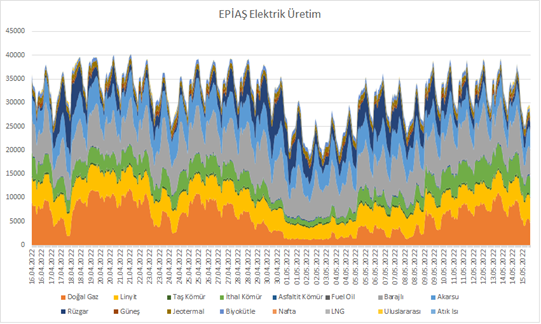
\includegraphics{amount.png}
\caption{amount.png}
\end{figure}

    The one-month period from 16th of April to 16th of May 2022 includes
Ramadan holiday where electricity demand is reduced. The market exchange
price, which is around the cap during workdays, drops during the holiday
period.

\begin{figure}
\centering
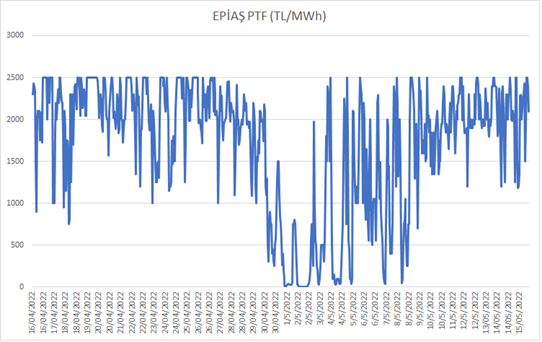
\includegraphics{price.png}
\caption{price.png}
\end{figure}

    \hypertarget{energy-flows-for-electricity-generation-with-storage}{%
\subsection{Energy flows for electricity generation with
storage}\label{energy-flows-for-electricity-generation-with-storage}}

\begin{figure}
\centering
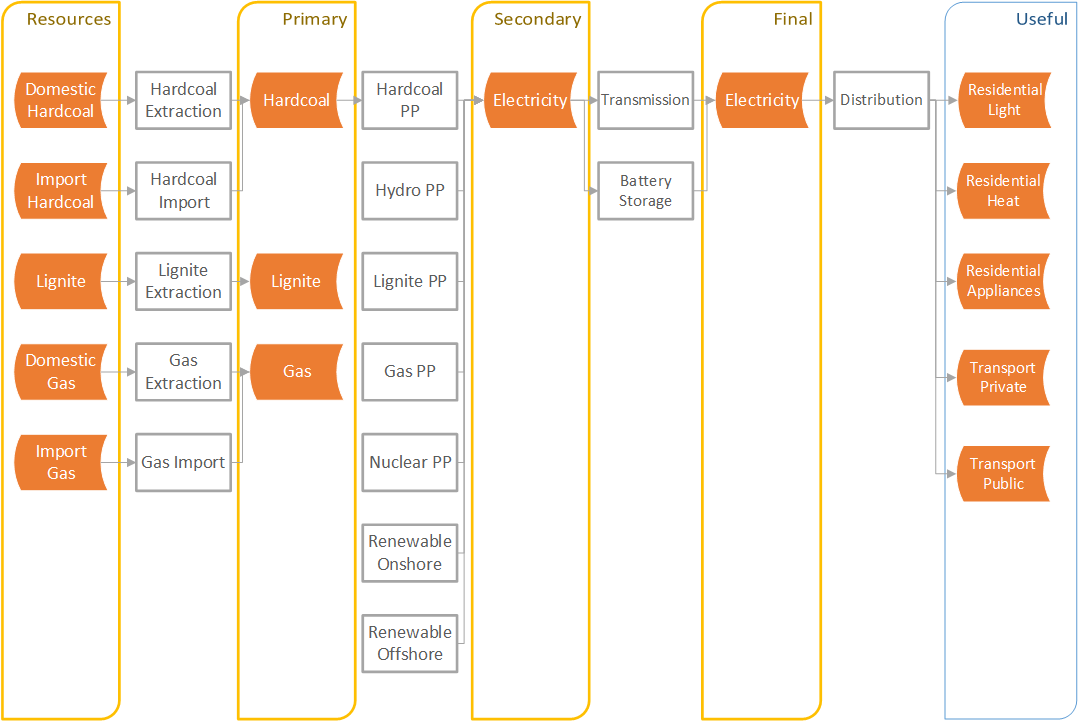
\includegraphics{electricity_flow.png}
\caption{electricity\_flow.png}
\end{figure}

    \hypertarget{further-steps}{%
\subsection{Further steps}\label{further-steps}}

\begin{itemize}
\tightlist
\item
  Include data from recent academic (peer-reviewed) studies based on the
  net-zero target of Turkey
\item
  Extract meta-data for emissions and related temperature increase using
  \textbf{MAGICC} emulator
\item
  Develop a model for the low carbon transition of the electricity
  sector
\item
  Test the hypothesis for utilizing hydrogen and battery storage as a
  market solution for low carbon transition
\end{itemize}

    \hypertarget{questions}{%
\subsection{Questions?}\label{questions}}

Take a look at our
\href{https://github.com/gorkemgungormetu/turkish_energy_and_climate_pathways.git}{GitHub
repository}!

    \begin{tcolorbox}[breakable, size=fbox, boxrule=1pt, pad at break*=1mm,colback=cellbackground, colframe=cellborder]
\prompt{In}{incolor}{55}{\boxspacing}
\begin{Verbatim}[commandchars=\\\{\}]
\PY{n}{df}\PY{o}{.}\PY{n}{to\PYZus{}excel}\PY{p}{(}\PY{l+s+s1}{\PYZsq{}}\PY{l+s+s1}{data\PYZus{}export.xlsx}\PY{l+s+s1}{\PYZsq{}}\PY{p}{)}
\end{Verbatim}
\end{tcolorbox}


    % Add a bibliography block to the postdoc
    
    
    
\end{document}
